\documentclass[letterpaper,11pt,twoside]{book} 

%Configuración inicial
\usepackage[spanish]{babel} %español 
\usepackage[utf8]{inputenc} %acentos
\usepackage{amsmath,float,graphicx,gensymb} %ecuaciones/imágenes
\usepackage{svg} %gráficos vectoriales escalables
\usepackage{afterpage} %salto de página
\usepackage{ragged2e} %guiones de alineación de página 
\usepackage[margin=1in]{geometry} %tamaños de margen
\usepackage[sc]{mathpazo} %fuente
\newcommand{\grad}{$^{\circ}$} %grados
\usepackage{hyperref} %referencias navegables
\usepackage{upgreek} %diferentes letras griegas
\decimalpoint %usar punto en vez de la coma por default en el paquete de idioma español

%Características de las referencias
\usepackage[round]{natbib}
\bibliographystyle{apalike}


%Comandos para cambiar la posición de los títulos de capítulo
\usepackage[compact]{titlesec}
\titleformat{\chapter}[display]
{\normalfont\huge\bfseries}{\chaptertitlename\ \thechapter}{20pt}{\Huge}
\titlespacing*{\chapter}{0pt}{-15mm}{40pt}
\setlength{\parindent}{0cm}


%Comandos para páginas en blanco
\newcommand\blankpage{%
    \null
    \thispagestyle{empty}%
    \addtocounter{page}{-1}%
    \newpage}
    
\begin{document}

	\include{portada}
	\afterpage{\blankpage}	
	\let\cleardoublepage\clearpage
	
	%Frase	
	\chapter*{}
	\begin{flushright}
	\pagestyle{empty}
	\thispagestyle{empty}
	\textit{per aspera ad astra}
	\end{flushright}
	\afterpage{\blankpage}
	
	\pagenumbering{roman}
	
	\chapter{Agradecimientos}

A la Dra. Graciela Raga y el Dr. Luis Ladino del grupo de Interacción Micro y Mesoescala del Centro de Ciencias de la Atmósfera por brindarme un segundo hogar propicio para desarrollar mi investigación con todas las libertades intelectuales y las facilidades económicas y materiales. Mi estancia en su grupo me ha permitido reflexionar acerca de que la ciencia es mucho más que academia y producción, también es comunidad, autocrítica y sensibilidad. Sin el apoyo económico de la Dra. Graciela Raga a través del Programa de Ayudantes de Investigador del Consejo Nacional de Ciencia y Tecnología este trabajo de carácter autogestivo no hubiera podido ser. Sin la guía y los consejos del Dr. Luis Ladino tantas ideas en el aire no habrían podido aterrizar.\\

A Emily Rivera y David \textit{Tiger} León por enseñarme que los conocimientos científicos no pertenecen más que a la propia naturaleza pero que las ideas críticas con reconocimiento a sus autores son la base permanente que nos permite tratar de explicar nuestro universo desde nuestro particular campo de acción. Siéntanse orgullosos y vean hasta dónde ha llegado su idea que nació en una tarde cualquiera de hace cuatro años.\\

A mi director de tesis, el Dr. Héctor Solano del Consorcio para el Estudio de Zonas Metropolitanas por haber creído en el valor de mi propuesta y brindarme en el acto, total libertad creativa en el diseño de mi investigación, sin ningún tipo de interés personal más que la motivación compartida por hacer frente al problema de contaminación lumínica en mi ciudad, la Ciudad de México. Gracias por introducirme a una vastedad de pormenores teóricos y técnicos de la investigación de la luz artificial durante la noche y permitirme acceder al modelo \textit{SkyGlow} bajo el consentimiento de su autor, el Dr. Miroslav Kocifaj de la Academia Eslovaca de Ciencias, para dar respuesta a mis más viscerales preguntas, mismas que me ayudó a traducir en términos científicos rigurosos.\\

A la Reserva Ecológica del Pedregal de San Ángel por haberme brindado espacio y reflexiones en mi formación personal más allá de la educación tan rígida que recibimos en las aulas. Reconocimientos especiales se merecen Marcela Pérez, Hilda Díaz, Merly Fabila y Néstor Chavarría por generar y compartir espacios universitarios en que podemos abordar tantas cuestiones tradicionalmente reprimidas: llamar por su nombre, capitalismo, al sistema responsable de la actual crisis mundial, expresar nuestros sentimientos como parte fundamental de nuestro actuar, visibilizar nuestra identidad sexual y voltear, por fin, el rostro a esos defensores de la humanidad sepultada bajo la violencia del poder, el odio a lo diferente y la competencia por ser <<el mejor>>. Esos defensores anónimos son los colaboradores que se saltan clases para recoger basura del pedregal, las feministas que dan y dedican su vida por los derechos de las mujeres, los zapatistas que luchan por su territorio y cada uno de los migrantes e indígenas del mundo.\\

A \textit{Las Tachas}, Lilia de la Cruz, Alejandra Argüelles e Ivonne Castillo por todos los momentos compartidos en el pedregal: las noches en que alcanzamos a ver muchas estrellas dentro de la Zona Núcleo Oriente, esperamos toda la tarde a los murciélagos, medimos colas de ratones en campo, nuestros ojos brillaron al contarle a cientos de personas acerca de la magia que tiene el pedregal y, en especial, cuando su discurso en defensa del Molotito hizo brotar mis lágrimas de orgullo.\\  

A mis amigos de la Facultad de Ciencias que me sonrojaron con su presencia, me maravillaron con sus ideas, me acompañaron en la comida, respetaron sin interrogaciones mi decisión de no beber, me abrazaron en la crisis de no saber y escucharon todas las inquietudes del mundo académico, filosófico y del amor que me dejaban sin dormir. Las buenas calificaciones no sirven más que para dedicárselas a cada uno de ustedes por la paciencia que tuvieron al explicarme lo que se me dificultaba y por la entrega que le dieron a las tareas y proyectos que elaboramos juntos. Gracias Jaime \textit{Jimbo} González, Delfina \textit{Mina} Cruz, Andrea Anguiano, Aarón Contreras, Alejandro Vega y a mis \textit{Repoixs} Andrea García, Zyanya Díaz, Diana \textit{Repoio} Morales e Iván Pineda.\\

A mis \textit{CCAmigos} por todo su apoyo profesional y por ser la razón de estar de buenas todo el día en el Centro de Ciencias de la Atmósfera: a Sandrita Porras, mi alma gemela, a Diego Cabrera por todas las carcajadas, a Carito Ramírez, Fernanda Córdoba, Montserrat Silva, Orlando Peña y a Daniel Pretelín (gracias por agradecerme en tus agradecimientos, amigo).\\

A mis amigos de siempre por ser el pilar que no ha dejado que mi crisis existenciales me derriben, ustedes me han enseñando el supremo placer de vivir. Gracias a Memo Papaya por enseñarme que el amor es incondicional, a Dianita Colín, Marianita Quiroz y Ayleen Aguilar por mostrarme el camino a mi feminidad, a Alan Benitez, Alberto Fiesco y Abraham Almaguer por compartir conmigo las grandes pasiones de nuestras vidas: la teología, la música y la fotografía, respectivamente.\\

Al erario de México y a la Universidad Nacional Autónoma de México 

Aquí agregaré agradecimientos a familia (núcleo y Xalapa), Fabi, Alejandro Zenteno, profesores (Marco Antonio Miramontes, Diego Alfaro y Fernando García), programa PAECI, erario México, UNAM, Ivonne del CCA, investigadores de Barcelona (UPC Y UB), sinodales, a la AGU y a las alcaldías por los datos facilitados de alumbrado público a través del InfoDF.
	\afterpage{\blankpage}
	
	\chapter{Abreviaturas}

\begin{itemize}

\item[$\cdot$] \textbf{AERONET} \textit{AErosol RObotic NETwork}

\item[$\cdot$] \textbf{ANP} Áreas Naturales Protegidas

\item[$\cdot$] \textbf{AOD} \textit{Aerosol Optical Depth}

\item[$\cdot$] \textbf{ASY} \textit{Asymmetry Parameter}

\item[$\cdot$] \textbf{CEF} \textit{City Emission Function}

\item[$\cdot$] \textbf{CU} Ciudad Universitaria

\item[$\cdot$] \textbf{CL} Contaminación Lumínica

\item[$\cdot$] \textbf{DNB} \textit{Day/Night Band}

\item[$\cdot$] \textbf{EC} Especies Carbonosas: carbón elemental + carbón orgánico

\item[$\cdot$] \textbf{EE} Espectro Electromagnético

\item[$\cdot$] \textbf{FP} Condiciones de Fondo Promedio

\item[$\cdot$] \textbf{GEF} \textit{Garstang Emission Function}

\item[$\cdot$] \textbf{GEI} Gases de Efecto Invernadero

\item[$\cdot$] \textbf{IDA} \textit{International Dark-Sky Association}

\item[$\cdot$] \textbf{LED} \textit{Light Emitting Diode}

\item[$\cdot$] \textbf{LGEEPA} Ley General de Equilibrio Ecológico y Protección al Medio Ambiente

\item[$\cdot$] \textbf{MODS} Método de Órdenes de Dispersión Sucesivos

\item[$\cdot$] \textbf{NOAA} \textit{National Oceanic and Atmospheric Administration}

\item[$\cdot$] \textbf{OAN} Observatorio Astronómico Nacional

\item[$\cdot$] \textbf{REPSA} Reserva Ecológica del Pedregal de San Ángel

\item[$\cdot$] \textbf{SEMARNAT} Secretaría del Medio Ambiente y Recursos Naturales

\item[$\cdot$] \textbf{SI} Sistema Internacional de Unidades

\item[$\cdot$] \textbf{SQM} \textit{Sky Quality Meter}

\item[$\cdot$] \textbf{SSA} \textit{Single Scatter Albedo}

\item[$\cdot$] \textbf{UNAM} Universidad Nacional Autónoma de México

\item[$\cdot$] \textbf{UNESCO} \textit{United Nations Educational, Scientific and Cultural Organization}

\item[$\cdot$] \textbf{VIIRS} \textit{Visible Infrared Imaging Radiometer Suite}
			
\end{itemize}
	\afterpage{\blankpage}
	
	\chapter{Resumen}

Las ciudades albergan a la mayoría de las poblaciones humanas a nivel mundial \citep{Zari2018}. El caso de estudio de esta tesis es el de la Ciudad de México, la cual actualmente concentra cerca de 9 millones de habitantes \citep{INEGI2015} y está inmersa en la Zona Metropolitana del Valle de México, con una población total de alrededor de 22 millones de habitantes \citep{OCDE2015}. Esta aglomeración implica serias consecuencias ambientales y hace a la región altamente dependiente de subsidios: con sólo 7\% de la población total de México, en la Ciudad de México se consume casi un tercio del petróleo demandado en el país y 6\% del total de la energía eléctrica \citep{SENER2013}.\\

Como consecuencia de una dinámica centralista, en la Ciudad de México se cuenta con alrededor de 600 mil luminarias públicas funcionando en vías primarias y secundarias; por la cantidad y características de tales puntos de luz, se puede hipotetizar que la capital del país actualmente se está enfrentando a otro problema ambiental más: la contaminación lumínica (CL).\\

La CL es el conjunto de efectos de difusión, en la atmósfera nocturna, de la luz producida por fuentes artificiales que alteran las condiciones originales de luminosidad; estos efectos se producen por la emisión del flujo luminoso en intensidades, direcciones, rangos espectrales u horarios innecesarios, siendo algunos de los más apremiantes la degradación de los socioecosistemas y, más específicamente, afectación a la población humana en temas de uso sustentable de energía, salud y ética \citep{AtlasREPSA}, \citep{LibroCL}, \citep{Stone2017}.\\

Aunque este tipo de contaminación comenzó a considerarse un problema ambiental desde principios de la década de 1960 \citep{LibroCL}, hasta ahora no se han realizado estudios referentes al tema en ninguna ciudad del país. Esta tesis es, pues, el primer antecedente de la estimación de los niveles de contaminación lumínica en la Ciudad de México, con el uso del modelo teórico de dispersión de la luz en la atmósfera \textit{SkyGlow} desarrollado por Kocifaj \citep{Kocifaj2007}.\\

Aquí se agregarán los resultados encontrados a grandes rasgos.


	\afterpage{\blankpage}
	
	\chapter{Productos}

\textbf{\begin{Large}
Congresos
\end{Large}}\\

\textbf{Joshua Iván Muñoz Salazar} \textit{Efectos de la contaminación lumínica en especies de hábito nocturno}. En Noche de las Estrellas: 3 de diciembre de 2016. Universidad Nacional Autónoma de México, Ciudad de México, México.\\

\textbf{Joshua Iván Muñoz Salazar} y Héctor Antonio Solano Lamphar. \textit{Radiación lumínica en la atmósfera}. En Tercer Simposio de Ciencias de la Tierra: 6 - 8 de noviembre de 2017. Facultad de Ciencias, Universidad Nacional Autónoma de México, Ciudad de México, México.\\

\textbf{Joshua Iván Muñoz Salazar} y Héctor Antonio Solano Lamphar. \textit{Determinación de propiedades ópticas de nubes con base en su contenido de agua líquida}. En XII Congreso Internacional de Meteorología: 13 - 16 de noviembre de 2018. Universidad Veracruzana, Veracruz, México.\\

\textbf{Joshua Iván Muñoz Salazar} y Héctor Antonio Solano Lamphar. \textit{Contaminación lumínica: otra dimensión para la mitigación del calentamiento global}. En 8º Congreso Nacional de Investigación en Cambio Climático: 9 y 10 de octubre de 2018. Centro de Ciencias de la Atmósfera, Universidad Nacional Autónoma de México, Ciudad de México, México.\\

\textbf{Joshua Iván Muñoz Salazar} y Héctor Antonio Solano Lamphar. \textit{Contaminación lumínica en la Ciudad de México}. En 8º Coloquio de Estudiantes. Causas, efectos y soluciones de la crisis ambiental: 21 de noviembre de 2019. Centro Interdisciplinario de Investigaciones y Estudios sobre Medio Ambiente y Desarrollo, Instituto Politécnico Nacional, Ciudad de México, México.\\

\textbf{\begin{Large}
Estancias de investigación
\end{Large}}\\

\textbf{Grupo de Estudios Luminotécnicos}. Departamento de Ingeniería de Proyectos y Construcción. Escuela Técnica Superior de Ingeniería Industrial de Barcelona. Universidad Politécnica de Cataluña.\\

\textbf{Departamento de Astronomía y Meteorología}. Instituto de Ciencias del Cosmos. Universidad de Barcelona.\\

Diciembre 2018. Barcelona, España.










	\afterpage{\blankpage}

	\tableofcontents
	 
	\cleardoublepage
	\phantomsection
	\renewcommand\listfigurename{Índice de figuras}
    \addcontentsline{toc}{chapter}{\listfigurename}
	\listoffigures
	
	\cleardoublepage
	\phantomsection
	\renewcommand\listtablename{Índice de tablas}
    \addcontentsline{toc}{chapter}{Índice de tablas}
	\listoftables
	\afterpage{\blankpage}

	\mainmatter %comienza numeración arábiga
	
	\chapter{Introducción}


\section{Fundamentos teóricos de la luz}

\subsection{Radiación electromagnética}

La luz es radiación electromagnética que se propaga en forma de onda a través del espacio transportando energía radiante en el proceso. Está constituida por partículas elementales sin masa denominadas fotones \citep{Purcell&Morin2013}. Las propiedades de la luz están condensadas en el espectro electromagnético (EE) (Figura~\ref{espectroelectromagnetico}) con base en el número de oscilaciones de la onda por unidad de tiempo (frecuencia, $\nu$) y la distancia lineal entre dos puntos equivalentes de ondas sucesivas (longitud de onda, $\lambda$).\\

\begin{figure}
  \centering
    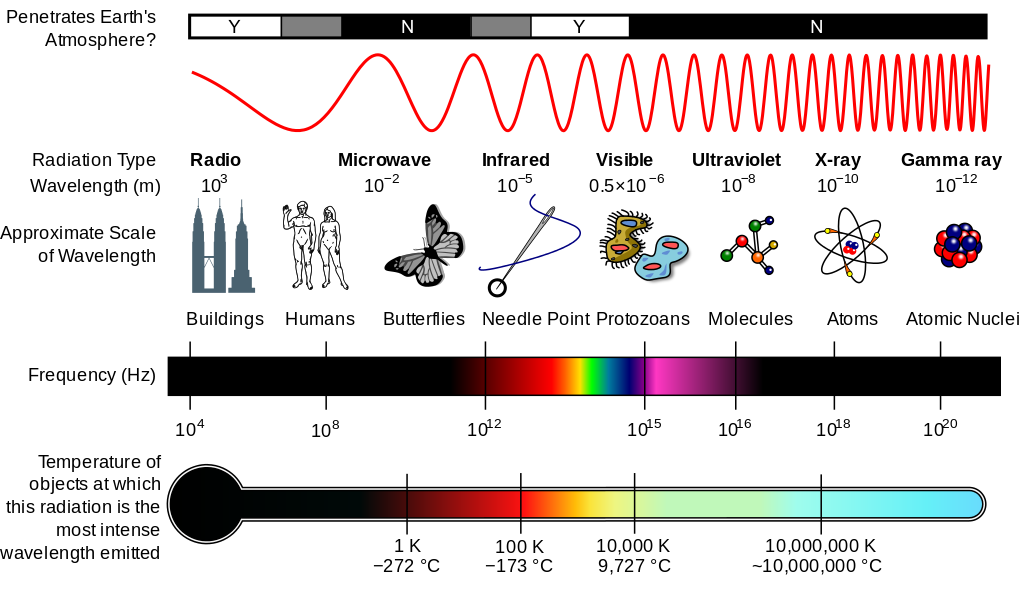
\includegraphics[width=0.9\textwidth]{espectroelectromagnetico}
  \caption{Espectro electromagnético \citep{NASA2007}}
  \label{espectroelectromagnetico}
\end{figure}

Una de las propiedades de la luz de interés para este trabajo en la región visible del EE ($\sim$ 350-800 nm) es la temperatura de color ($T$)  que está definida a partir de la Ley de desplazamiento de Wien \citep{Halliday&Resnick2008}. Esta ley explica la relación inversa entre la longitud de onda en la que se produce el pico de emisión de un cuerpo negro ($\lambda_{max}$) y $T$:

\begin{equation}
\lambda_{max} = \dfrac{b}{T}
\end{equation}

Donde $b = 2.897...\e{-3}$ m K, es denominada la constante de Wien. Un cuerpo negro es un objeto ideal que absorbe y emite toda radiación electromagnética; en equilibrio termodinámico y térmico, emite radiación térmica sólo con dependencia en su temperatura.\\

En la \textbf{\autoref{sec:luzartificial}} y en la \textbf{\autoref{sec:contaminacionluminica}} se presenta la aplicación del concepto de temperatura de color para la clasificación del color de las fuentes de luz y su implicación biológica en los humanos.\\

\subsection{Propiedades ópticas}

La óptica es el campo de la física que se encarga de estudiar la interacción de la luz con la materia. En la  \textbf{Tabla \ref{tab:propiedadesopticas}} se resumen las principales propiedades ópticas.

\begin{table}[]
\centering
\caption{Propiedades ópticas de la luz  \citep{Born&Wolf2003}}
\label{tab:propiedadesopticas}
\resizebox{0.9\textwidth}{!}{%
\begin{tabular}{|l|l|l|}
\hline
\textbf{\textbf{Propiedad}} & \textbf{} & \textbf{\textbf{Descripción}} \\ \hline
Absorción &  & La luz es captada en el objeto y aumenta su energía térmica \\ \hline
Transmisión &  & La luz atraviesa el objeto sin cambio de dirección ni intensidad \\ \hline
Dispersión &  & La luz es captada en el objeto y se re-emite con diferente dirección e intensidad \\ \cline{2-3} 
 & Rayleigh & Dispersión elástica (conserva energía) en que la longitud de onda de la luz \\
 &  & incidente es mucho mayor que el tamaño del objeto \\ \cline{2-3} 
 & \multicolumn{1}{c|} {Mie} & Dispersión elástica en que la longitud de onda de la luz incidente es similar \\
 &  & al tamaño del objeto \\ \hline
Reflexión &  & La luz se desvía al chocar con el objeto con un ángulo igual al de incidencia \\ \hline
Refracción &  & La luz cambia de dirección y velocidad al atravesar por un medio diferente \\ \hline
\end{tabular}%
}
\end{table}

\newpage

\subsection{Unidades de medición}

Existen dos campos de estudio que se encargan de la medición de la luz: la fotometría y la radiometría. La fotometría se encarga de medir la luz con base en la sensibilidad de la vista humana. Por otro lado, la radiometría mide la luz abarcando todas las longitudes de onda del EE. Al ser de carácter general este trabajo, en la \textbf{Tabla \ref{tab:unidadesradiometria}} se muestran las unidades del Sistema Internacional de Unidades (SI) utilizadas en radiometría.\\

Para estudios enfocados en los niveles de luminosidad en ecosistemas y su influencia en cada uno de sus componentes con base en su sensibilidad, es fundamental utilizar medidas fotométricas (véase el \textbf{\autoref{chap:recomendaciones}}).


\begin{table}[htb]
\centering
\caption{Unidades del SI utilizadas en radiometría \citep{Jurgen1968}}
\label{tab:unidadesradiometria}
\resizebox{\textwidth}{!}{%
\begin{tabular}{|l|l|l|}
\hline
\textbf{\textbf{Magnitud física}} & \textbf{\textbf{Unidad del SI}} & \textbf{\textbf{Notas}} \\ \hline
Energía radiante (Q) & J & Energía \\ \hline
Flujo radiante ($\Phi$) & W & Energía radiada por unidad de tiempo (potencia) \\ \hline
Intensidad radiante (I) & W sr$^{-1}$ & Potencia por ángulo sólido \\ \hline
Irradiancia (E) & W m$^{-2}$ & Potencia incidente por superficie \\ \hline
Emitancia radiante (M) & W m$^{-2}$ & Potencia emitida por superficie de la fuente radiante \\ \hline
Radiancia (L) & W sr$^{-1}$  m$^{-2}$ & Potencia por ángulo sólido y por superficie \\ \hline
Radiancia espectral ($L_{\lambda}$) & W sr$^{-1}$  m$^{-3}$ & Potencia por ángulo sólido, por superficie y por longitud de onda \\ \hline
\end{tabular}%
}
\end{table}

\newpage

\section{Brillo del cielo nocturno}
\label{sec:brillocielonocturno}

\subsection{Componentes del brillo del cielo nocturno}
\label{subsec:componentesbrillocielo}

En la \textbf{Tabla \ref{tab:componentesbrillo}} se describen los principales componentes del brillo total del cielo nocturno sin Luna $(I_{tot})$ tal como \cite{Leinert1998} lo reportan para el rango del ultravioleta lejano ($\sim$ 100 nm) al infrarrojo lejano ($\sim$ 200 $\mu$m).


\begin{table}[htb]
\centering
\caption{Componentes del brillo del cielo nocturno \citep{Leinert1998}}
\label{tab:componentesbrillo}
\resizebox{\textwidth}{!}{%
\begin{tabular}{|l|l|}
\hline
\textbf{\textbf{Componente}} & \textbf{\textbf{Descripción}} \\ \hline
Brillo del aire ($I_A$) & \begin{tabular}[c]{@{}l@{}}Excitación de átomos de oxígeno y nitrógeno de la atmósfera superior\\ por su interacción con la radiación solar\end{tabular} \\ \hline
Luz zodiacal ($I_{ZL}$) & Dispersión de la radiación solar en partículas de polvo interestelar \\ \hline
Luz estelar ($I_{ISL}$) & La luz de las estrellas en su conjunto \\ \hline
Luz difusa galáctica ($I_{DGL}$) & Luz emitida y dispersada por partículas de polvo de la galaxia \\ \hline
Luz de fondo extragaláctica ($I_{EBL}$) & Luz producida por galaxias o cúmulo de galaxias \\ \hline
Luz artificial ($I_{SCA}$) & Luz artificial dispersada en la tropósfera \\ \hline
\end{tabular}%
}
\end{table}

La suma de tales componentes (excepto luz artificial, netamente de origen antropogénico) se considera de origen natural y es susceptible de ser atenuada por acción de la atenuación atmosférica. De acuerdo con esta clasificación, el brillo total del cielo nocturno puede calcularse a partir de la siguiente ecuación:

\begin{equation}
I_{tot} = (I_A + I_{ZL} + I_{ISL} + I_{DGL} + I_{EBL})\:e^{-\tau} + I_{SCA}
\end{equation}

\vspace{2mm} 

Donde $\tau$ es el coeficiente de atenuación atmosférica que depende de la longitud de onda, la distancia cenital (la distancia angular del cuerpo celeste con respecto al cenit), la altura sobre el nivel del mar del observador y las condiciones atmosféricas.\\ 

La definición matemática del brillo total del cielo nocturno nos permite inferir que las principales contribuciones se deben al brillo del aire y a la luz zodiacal; estimaciones experimentales confirman este comportamiento reportando mediciones de radiancia de hasta 10$^{-4}$ W sr$^{-1}$  m$^{-2}$ atribuibles al brillo del aire \citep{Leinert1998}.\\ 

\subsection{Variación natural del brillo del cielo nocturno por influencia de la Luna}

La luz lunar percibida en la Tierra es resultado de la reflexión de la luz solar y, en menor medida, terrestre en la superficie de la Luna. El albedo lunar es 0.136 lo que significa que refleja 13.6\% del total de la radiación incidente \citep{Matthews2008}. La cantidad de luz lunar varía hasta en tres órdenes de magnitud a lo largo del mes de acuerdo con el ciclo lunar \citep{Kyba2017}.\\

En condiciones atmosféricas despejadas y de nula luz artificial, la luz lunar es la principal responsable del brillo total del cielo nocturno ya que, típicamente, los valores de brillo del aire son hasta tres órdenes de magnitud más pequeños que los reportados para la luz lunar \citep{Hanel2018}.\\

\newpage

Es importante tomar en cuenta la advertencia de \cite{Kyba2017} quienes reportan que en la literatura científica existen datos erróneos de luz lunar y hacen visible la necesidad de una publicación que reporte valores típicos de referencia de luz lunar a través de estudios de largo plazo (al menos de un año) en localidades sin influencia de luz artificial.\\ 

Tomando en cuenta las consideraciones anteriores, para efectos de este estudio centrado en la luz artificial, se procede a despreciar los términos de luz de origen natural en la ecuación de brillo total del cielo nocturno sin Luna, reduciéndose entonces a:

\begin{equation}
I_{tot} = I_{SCA}
\end{equation}\\


\subsection{Variación natural del brillo artificial del cielo nocturno por influencia de las condiciones atmosféricas}

\subsubsection{Propiedades ópticas del aerosol atmosférico}
\label{subsubsec:propiedadesopticasaerosol}


La concentración de aerosol atmosférico depende principalmente de emisiones naturales y antropogénicas, patrones de circulación sinóptica, meteorología local y características topográficas \citep{Carabali2017}.\\

\cite{Garstang1991} describió por primera vez la dispersión de la luz artificial por acción del aerosol atmosférico. Posteriormente \cite{Kocifaj2007} verifica que el aerosol atmosférico puede amplificar o reducir el brillo del cielo nocturno con base en las propiedades ópticas de bulto descritas a continuación.\\

\textit{\textbf{Espesor óptico de aerosol (AOD)}}\\

El AOD es una cantidad adimensional que representa la atenuación atmosférica de la luz por el aerosol atmosférico integrada verticalmente en toda la columna atmosférica. La diferencia de potencial ($V$) medido por un fotómetro solar es proporcional a la radiancia espectral ($L_{\lambda}$) que es captada por el instrumento en la superficie \citep{Holben1998}. El espesor óptico total ($\tau_{TOT}$) puede calcularse a partir de la siguiente ecuación conocida como la ley de Beer-Lambert-Bouguer:

\begin{equation}
V(\lambda) = V_0(\lambda)\:d^{2} \:e^{-\tau_{TOT}\: m}
\end{equation}

Donde $V$ es la diferencia potencial medida en una longitud de onda dada $\lambda$, $d$ es la tasa entre el promedio y la distancia real Tierra-Sol y $m$ es la masa óptica de aire. La masa óptica de aire es la tasa entre la masa de aire que la luz solar atraviesa hasta la superficie de la Tierra y la masa de aire que atravesaría si la incidencia fuera vertical.\\

Otros constituyentes atmosféricos pueden dispersar la luz y, por lo tanto, deben de considerarse en el cálculo del AOD \citep{Holben1998} tal y como se muestra en la siguiente ecuación:

\begin{equation}
\tau (\lambda)_{Aerosol} = \tau (\lambda)_{TOT} - \tau (\lambda)_{agua} - \tau (\lambda)_{Rayleigh} - \tau (\lambda)_{O_3} - \tau (\lambda)_{NO_2} - \tau (\lambda)_{CO_2} - \tau (\lambda)_{CH_4}
\end{equation}

\newpage

\textit{\textbf{Parámetro de Angstrom}}\\

La distribución por tamaño del aerosol atmosférico puede ser estimada a través del Parámetro de Angstrom $(\alpha)$ \citep{Holben1998} definido a partir de la siguiente ecuación:

\begin{equation}
\alpha (\lambda_1, \lambda_2) = \frac { -ln (\frac{\tau_\lambda_2}{\tau_\lambda_1})}{ ln(\frac{\lambda_2}{\lambda_1})}
\end{equation}

Donde $\tau_\lambda_1$ y $\tau_\lambda_2$ son el AOD en las longitudes de onda $\lambda_1$ y $\lambda_2$ respectivamente. Típicamente los valores de $\alpha$ varían entre -2 y 2.  $\alpha$ $>$ 1, indica que el modo fino de aerosol atmosférico es dominante mientras que  $\alpha$ $<$ 1 indica que el modo grueso es el más abundante \citep{Carabali2017}.\\

\textit{\textbf{Parámetro de Asimetría (ASY)}}\\

Su valor es una medida de la dirección de la dispersión de la luz. Está definido como el promedio del coseno del ángulo de dispersión $\theta$ ponderado por intensidad de la luz:

\begin{equation}
ASY = < cos \theta > = \frac{1}{2} \int_{0}^{\pi} sen (\theta) cos(\theta) P(\theta) d\theta
\end{equation}

Con $P(\theta)$ la función de fase de dispersión que describe la dispersión de la luz dependiente del ángulo:

\begin{equation}
P(\theta) = \frac{4\pi}{\sigma_{SCA}} \frac{d\sigma_{SCA}}{d\theta}
\end{equation}

Donde $\sigma_{SCA}$ es la sección transversal de dispersión:

\begin{equation}
\sigma_{SCA} = \frac{\pi D^{2}}{4} Q_{SCA}
\end{equation}

Con $D$ el diámetro de la partícula y $Q_{SCA}$ la eficiencia de dispersión (cuánta energía absorbida es dispersada).\\

Cuando ASY = 1, toda la luz es dispersada hacia adelante; ASY = 0, indica una dispersión isotrópica \citep{Solano2015}.
\\

\textit{\textbf{Albedo de Dispersión Simple (SSA)}}\\

Este parámetro relaciona los coeficientes de dispersión ($\epsilon_{SCA}$) y absorción ($\epsilon_{ABS}$) \citep{Foot1987} como muestra la ecuación:

\begin{equation}
SSA = \frac{\epsilon_{SCA}}{\epsilon_{SCA} + \epsilon_{ABS}}
\end{equation}


Los coeficientes de dispersión $\epsilon$ se obtienen:

\begin{equation}
\epsilon = N \sigma
\end{equation}

Con $N$ la concentración de partículas de tamaño $D$. El valor del SSA es representativo de las propiedades de absorción de la luz del aerosol atmosférico. Cuando el valor del SSA es cercano a 1 es un indicativo que el aerosol en cuestión refleja más luz, mientras que, para el aerosol más absorbente, el valor del SSA es cercano a 0.\\

\subsubsection{Propiedades ópticas de las nubes}

\cite{Twomey1967} desarrolló por primera vez una teoría de dispersión de la luz debido a la nubosidad. Estudios más recientes \citep{Kocifaj2007}, \citep{Solano2014}, \citep{Solano2015}, han encontrado cambios significativos en el brillo del cielo por la dispersión de luz artificial por acción de la nubosidad. Las nubes son un medio dispersivo complejo, esto es, que poseen diferentes constituyentes con diferente índice refractivo complejo $(\underline{n})$ definido como:

\begin{equation}
\underline{n} = n + i k
\end{equation}

\vspace{2mm} 

Donde $n$, la parte real de la ecuación, indica la velocidad de la luz dentro de un medio y la parte imaginaria $k$ es el coeficiente de atenuación de la luz dentro del medio en cuestión \citep{Born&Wolf2003}. Los valores de la parte imaginaria del índice refractivo complejo para las gotitas de nube y los cristales de hielo que forman las nubes son muy bajos de acuerdo con \cite{Solano2015}.\\

Tomando en cuenta lo anterior, \cite{Solano2015} consideran a las nubes como cuerpos Lambertianos con albedo espectral variante para su estudio óptico. Un cuerpo Lambertiano es aquel que posee una superficie ideal que refleja la luz incidente de manera isotrópica, permitiendo así que el brillo de tal superficie sea la misma para el observador independientemente de su ángulo de visión \citep{Born&Wolf2003}.\\

El albedo espectral de las nubes depende principalmente de factores como la altitud de su base con respecto al observador y la microfísica incluyendo el contenido de agua líquida y la distribución por tamaño de las gotitas de nube \citep{Kocifaj2007}.\\ 

Resulta complicado medir el albedo espectral de las nubes durante la noche ya que la mayoría de los fotómetros que miden esta propiedad funcionan con base en niveles de radiación presentes sólo durante el día. Por esta razón, las simulaciones numéricas de la influencia de las nubes en el brillo del cielo nocturna resultan útiles \citep{Solano2015}.\\

Además, es importante mencionar que los factores que se toman en cuenta en la modelación teórica son capaces de reproducir diferentes comportamientos del brillo del cielo con respecto a la posición del observador, lo cual es deseable para la predicción del brillo del cielo nocturno influenciado por diferentes tipos de nubes \citep{Kocifaj2007}, \citep{Solano2015}.

\newpage

\section{Luz artificial}\\
\label{sec:luzartificial}

En esta sección se aborda la caracterización de la luz artificial (de origen netamente antropogénico). Para esta tesis se considera que el alumbrado público es el principal responsable del brillo del cielo nocturno ocasionado por luz artificial \citep{Solano2013b}.

\subsection{Fundamentos teóricos de las fuentes artificiales de luz}

El diseño de iluminación es una disciplina fundamental para la correcta iluminación en el alumbrado público, la cual requiere de colaboraciones con otros campos como la física, biología, ciencias de la Tierra, ingeniería y arquitectura. El reto es grande ya que una correcta iluminación debe ser sustentable, apropiada para su contexto y debe lograr ahorro económico \citep{LibroCL}, \citep{Globaldiscussion}. A continuación se presentan los conceptos físicos fundamentales detrás de la iluminación.\\


\textbf{Producción de luz}

Para la producción artificial de luz se necesita de una serie de transformaciones de energía. El primer paso es la generación de energía eléctrica. De acuerdo con \cite{Ramos2012}, la mayoría de la energía eléctrica consumida en México es generada a partir de la transformación de energía química por medio de la combustión de hidrocarburos.\\

Una vez generada la energía eléctrica, necesita ser transformada en energía radiante. Esto se logra por medio del mecanismo interno de la fuente de luz. Los mecanismos más utilizados son la termorradiación (radiación de un cuerpo caliente) y luminiscencia (radiación de cuerpo no caliente) \citep{LibroCL}. En la \textbf{\autoref{subsec:fuentesdeluz}} se abordan las particularidades de cada uno de estos mecanismos.\\


\textbf{Distribución espectral}

La cantidad de energía radiada en determinadas regiones del EE \citep{Solano2013}. En la \textbf{\autoref{subsec:fuentesdeluz}} se muestran los gráficos de distribución espectral para diferentes tipos de fuentes de luz artificial.\\

  
\textbf{Temperatura de color}

La temperatura de color define el color de una fuente de luz sólo si esta se asemeja a un cuerpo negro. La mayoría de las fuentes de luz tradicionalmente utilizadas (incandescentes) se asemejan a un cuerpo negro, mientras que para las que no cumplen con esa característica (de descarga y LED), se implementa la temperatura de color correlacionada \citep{LibroCL}.\\

Para efectos de evaluación de reproducción de color y confort se asocia una apariencia de color a los rangos de temperatura de color teniendo <<luz cálida>> para temperatura de color de hasta 3000 K, <<luz intermedia>> de 3000 - 5300 K y <<luz fría>> para temperaturas de color mayor a 5300 K \citep{Globaldiscussion}.\\


\textbf{Eficiencia}

Definida para estudios fotométricos, se trata de la cantidad de flujo luminoso (visible) emitido por una fuente de luz por unidad de potencia consumida. La unidad del flujo luminoso es el lumen (lm), el equivalente fotométrico del flujo radiante. No es posible obtener una eficiencia de 100$\%$ debido a las pérdidas ocasionadas por disipación calorífica y radiaciones no visibles para el humano \citep{LibroCL}.


\subsection{Fuentes de luz artificial}
\label{subsec:fuentesdeluz}

Existen tres principales tipos de fuentes de luz artificial: incandescente, de descarga y diodo emisor de luz (LED, por sus siglas en inglés) (\textbf{Tabla \ref{tab:luzartificial}}), (Figura~\ref{distribucionespectral})  \citep{Solano2013b}, \citep{Eldvidge2010}, \citep{LibroCL}.\\

La iluminación incandescente es la más antigua y la más utilizada para interiores, su funcionamiento se basa en hacer pasar corriente eléctrica a través de un filamento, aumentando su temperatura hasta hacer que emita radiaciones visibles (termorradiación).\\

Por otro lado, la luz de descarga, utilizada ampliamente para alumbrado público, es generada por la excitación de un gas sometido a descargas eléctricas entre dos electrodos (luminiscencia).\\

Por último, el LED, que recientemente se ha comenzando a implementar en el alumbrado público, genera luz moviendo electrones de un semi-conductor sólido de un estado de alto nivel de energía a uno más bajo a través de la aplicación de una diferencia de potencial (electroluminiscencia).


\begin{table}[htb]
\centering
\caption{Principales fuentes de luz artificial}
\label{tab:luzartificial}
\resizebox{\textwidth}{!}{%
\begin{tabular}{|c|c|c|c|}
\hline
\textbf{Tipo} & \textbf{Fuente de luz} & \textbf{Temperatura de color (K)} & \textbf{Eficiencia (lm W$^{-1}$)} \\ \hline
Incandescente & Lámpara incandescente & 2700 & 8 - 18 (baja) \\ \hline
De descarga & Lámpara de sodio a baja presión (LPS) & 2000 & 180 (muy alta) \\ \cline{2-4} 
 & Lámpara de sodio a alta presión (HPS) & 2300 & 100 (alta) \\ \cline{2-4} 
 & Lámpara de halogenuros metálicos (MH) & 2800 - 5000 & 70 - 90 (alta) \\ \cline{2-4} 
 & Lámpara de vapor de mercurio (MV) & 3200 - 4000 & 60 (media) \\ \hline
LED & LED & 2700 - 5000 & 10 - 150 (baja) \\ \hline
\end{tabular}%
}
\end{table}


\begin{figure}[htb]
  \centering
    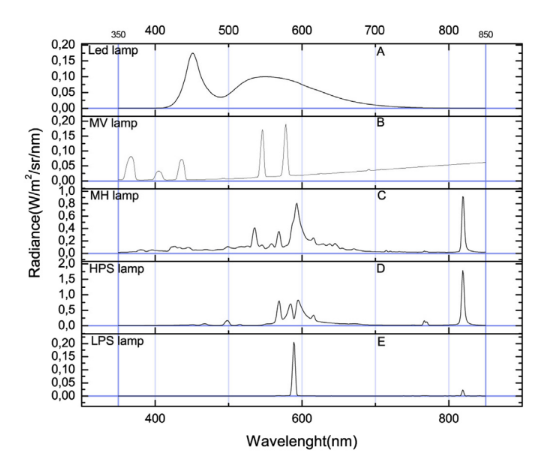
\includegraphics[width=100mm, scale=1]{distribucionespectral}
  \caption{Distribución espectral de A) LED, B) Vapor de mercurio, C) Halogenuros metálicos, D) Sodio a alta presión y E) Sodio a baja presión \citep{Solano2013b}}
  \label{distribucionespectral}
\end{figure}

\newpage

\subsection{Tipos de luminarias}
\label{subsec:luminarias}

Las luminarias son dispositivos que alojan y protegen la fuente de luz y reconducen su luz hacia donde se quiere iluminar \citep{LibroCL}. Para el caso del alumbrado público existen dos tipos: luminarias para vías principales (autopistas, carreteras) y luminarias para vías secundarias (calles) \citep{INFO2019}.\\

La forma en que la luminaria distribuye en el espacio la luz emitida por la fuente es fundamental en el efecto sobre el brillo del cielo nocturno. \cite{Marin2009} propone el ángulo entre la línea vertical de la fuente de luz y la línea máxima a la que ilumina (ángulo de apantallamiento) para garantizar un buen aprovechamiento de la luz y evitar que se desperdicie escapando hacia la atmósfera. El ángulo de apantallamiento ideal es por debajo de los 75\grad (A); para ángulos mayores a ese (B - E) existe afectación en diferente proporción al brillo del cielo nocturno (Figura~\ref{anguloapantallamiento}).


\begin{figure}[htb]
  \centering
    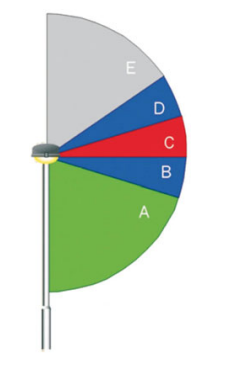
\includegraphics[width=30mm, scale=0.3]{anguloapantallamiento}
  \caption{Ángulo de apantallamiento de luminaria \citep{Marin2009}}
  \label{anguloapantallamiento}
\end{figure}


\subsection{Función de emisión urbana}
\label{subsec:funciondemisionurbana}

Las fuentes de luz artificiales (públicas y privadas) emiten luz en casi todas las direcciones \citep{Kocifaj2014}, \citep{Kocifaj2016}. Por lo tanto, la luz artificial emitida a la atmósfera se debe a la superposición de emisiones de las diferentes fuentes distribuidas en la superficie.\\

La distribución angular de la luz emitida por una ciudad es fundamental para la modelación del brillo del cielo nocturno ocasionado por luz artificial \citep{Kocifaj2014} esta distribución es caracterizada a través de una función de emisión parametrizada denominada Función de Emisión Urbana (CEF, por sus siglas en inglés) la cual depende de las características del sistema de iluminación de una ciudad \citep{Kocifaj2014}.\\

Debido a la falta, hasta la actualidad, de inventarios detallados de las fuentes de luz (públicas y privadas) y su naturaleza heterogénea, resulta extremadamente complicado obtener la CEF a través de estudios teóricos o experimentales \citep{Kocifaj2014}. \cite{Garstang1986} desarolló una aproximación semi-empírica para la estimación de la CEF, la cual es discutida en el \textbf{\autoref{chap:metodologia}}

\newpage

\section{Contaminación lumínica (CL)}\\
\label{sec:contaminacionluminica}

La CL es cualquier efecto negativo debido a la emisión de luz artificial en intensidades, direcciones, rangos espectrales u horarios innecesarios \citep{AtlasREPSA}, \citep{LibroCL}, \citep{Stone2017}.\\

En esta sección se presentan los argumentos que permiten afirmar que el brillo del cielo nocturno ocasionado por la luz artificial, es una fuente de CL en los socioecosistemas. Entiéndase contaminación como la alteración negativa de un sistema a través de la introducción de elementos físicos extraños \citep{AtlasREPSA}, \citep{LibroCL}.\\

Entiéndase un sistema como un conjunto de componentes interactuando en los que: 1) el comportamiento de cada componente tiene un efecto en el comportamiento del todo y, 2) el comportamiento de los componentes y sus efectos en el todo son interdependientes \citep{Avila2019}.\\

\subsection{El enfoque socioecosistémico}

Los seres humanos nombramos a la realidad natural de distintas maneras, las cuales poseen significados brutalmente diferentes de acuerdo con el fundamento filosófico con el que percibimos el planeta \citep{Avila2019}, \citep{Uribe2014}. Por ejemplo, las empresas extractivas denominan <<recursos naturales>> a tal realidad, los habitantes de una región, <<territorio>> y los científicos, <<ecosistema>>.\\

Con la aparición de la vida en la Tierra, surgieron los ecosistemas como un nivel de organización de la materia y la energía, en que el los sistemas físico-químicos (abióticos) y los sistemas bióticos interctuaron y evolucionaron de manera integrada. Sin embargo, con la emergencia de las sociedades y su organización con base en un lenguaje simbólico, nacen los socioecosistemas \citep{Avila2019}, \citep{Uribe2014}, \citep{Urquiza2015}.\\

Un socioecosistema es, por lo tanto, un sistema complejo (no lineal) y adaptativo que hace referencia a los procesos de acoplamiento e interacción entre los sistemas sociales (cultura, economía, organización social y política) y los ecosistemas \citep{Urquiza2015}.\\

Resulta fundamental, entonces, estudiar las problemáticas de contaminación ambiental desde el enfoque socioecosistémico. De esta manera se hace visible que, separar el nicho humano de la realidad natural, es el principal motor de la actual crisis ambiental. En este sentido, las Ciencias de la Tierra surgen como la disciplina integradora que, a través de la generación de conocimiento con un enfoque socioecosistémico, logra sembrar directrices en la construcción de la sustentabilidad.\\

\subsection{Importancia del ciclo día-noche en la evolución de la vida}

La duración del ciclo día-noche en la Tierra ha cambiado significativamente a lo largo de la historia geológica debido a la variación de la velocidad de rotación del planeta. La velocidad de rotación original de los planetas  es consecuencia de la conservación del momento angular que poseía la nebulosa interestelar que, al colapsar, dio origen al Sistema Solar hace aproximadamente 4600 Ma \citep{Greaves2005}.\\

Sin embargo, si la hipótesis del Impacto de Theia es correcta, es factible que la rotación primordial de la Tierra haya sido reconfigurada hace alrededor de 4500 Ma, cuando un cuerpo astronómico del tamaño de Marte, nombrado Theia, colisionó tangencialmente con nuestro planeta dando origen, además, a la Luna \citep{Stevenson1987}.\\

La velocidad de rotación actual de la Tierra debió comenzarse a perfilar hacia finales del periodo Criogénico (hace alrededor de 600 Ma), al mismo tiempo que los niveles de oxígeno y ozono estratosférico fueron óptimos para el surgimiento y desarrollo de vida más compleja (multicelular) en un evento conocido como \textit{la Radiación del Cámbrico}, durante el que se originaron y diversificaron la mayoría de los filos animales incluyendo el de los cordados, al que pertenecemos los humanos \citep{Conway2000}.\\

La mayoría de los organismos, incluyendo a los humanos, poseen ritmos circadianos que son controlados por el ciclo día-noche. Tales ritmos juegan un papel primordial en la regulación del metabolismo, el crecimiento y el comportamiento \citep{Dunlap1999}. Los fotoreceptores circadianos han estado presentes en la retina de los vertebrados desde hace aproximadamente 500 Ma, una vez que la duración del día se estableció en 24 horas \citep{Conway2000}, \citep{Longcore2006}.\\

Se ha encontrado que la proporción de especies vertebradas nocturnas que surgieron durante radiaciones evolutivas recientes es mayor con respecto a las antiguas (Figura~\ref{nocturnalidad}). Esto sugiere que la nocturnalidad es un importante paso en la evolución de los vertebrados \citep{Holker2010}. Sin embargo, no sólo la nocturnalidad es importante en los vertebrados, se estima que más del 60$\%$ de invertebrados son nocturnos \citep{Longcore2006}.


\begin{figure}[htb]
  \centering
    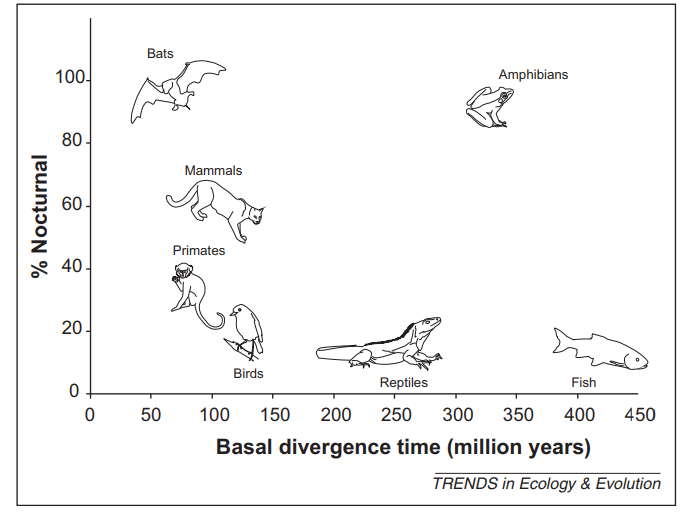
\includegraphics[width=95mm, scale=0.95]{nocturnalidad}
  \caption{Porcentaje de especies nocturnas de diferentes clases y órdenes de vertebrados con respecto a su origen \citep{Holker2010}}
  \label{nocturnalidad}
\end{figure}

Se teoriza que dada la alta permeabilidad de la piel de los anfibios y por ende, la susceptibilidad a las características de los nichos diurnos como la radiación solar, estos tuvieron que adoptar la nocturnalidad tempranamente \citep{Holker2010}.

\newpage

\subsection{Breve historia del uso y abuso de la luz artificial}\\
\\

Es sabido que el control regular del fuego por nuestros antepasados, desde hace aproximadamente 400 ka \citep{Dunbar2014}, fue fundamental en la evolución humana: la capacidad de cocinar alimentos mejoró la digestión y aprovechamiento de calorías, generando así el aumento de la masa cerebral; la llamas del fuego proveyeron protección de los predadores, permitiendo a los primeros humanos extender sus nichos ecológicos \citep{Wrangham2010}.\\

Por otro lado, la luz artificial del fuego extendió por primera vez la duración del día para las primeras sociedades. Las actividades nocturnas estuvieron lejos de ser económicamente productivas (exclusivamente diurnas); tales horas extras se dedicaron al canto, el baile, las ceremonias religiosas y a contar historias, lo que provocó una alteración en los ritmos circadianos de los primeros humanos \citep{Wiessner2014}.\\

Mientras que la observación de la Luna y las estrellas despertó el sentido de vulnerabilidad y preguntas sobre el origen del universo, las historias nocturnas crearon un espacio y contexto propicio para desarrollar órdenes más complejos de la conciencia de sí mismo, el entendimiento de los pensamientos y sentimientos de los otros, y la generación, regulación y transmisión de instituciones culturales \citep{Wiessner2014}.\\

Un esquema similar al de las primeras sociedades se siguió en los grupos humanos antiguos: los griegos, egipcios y chinos utilizaron lámparas de aceite en contextos religiosos a principios de la era común. Hasta antes de la Revolución Industrial (mediados del siglo XVIII) se utilizaron velas de cera y sebo con fines no económicos: como fuente de calor y fragancia e incluso para la cuenta del tiempo \citep{Duvall1988}.\\

Con la llegada de la Revolución Industrial como antecedente del capitalismo, los valores en torno a la luz artificial cambiaron radicalmente: la luz eléctrica se hizo necesaria para la iluminación de las jornadas nocturnas y el regreso a casa de los trabajadores. Se comenzaron a extender las horas productivas tradicionalmente restringidas durante el día para aumentar la producción \citep{Hudson1992}. Es fácil seguir esta tendencia hasta nuestros días al revisar las estadísticas que muestran que la mayor parte de energía eléctrica es utilizada para la industria y alumbrado público/privado \citep{Ramos2012}.\\ 


En conclusión, la lógica capitalista bajo la que vivimos ha transformado las horas nocturnas dedicadas antiguamente al descanso y a la realización de actividades espirituales y culturales en tiempo económicamente productivo gracias a la luz artificial producida e implementada en gran escala la cual, aún peor, está muy lejos de ser sustentable (véase \textbf{\autoref{subsec:consecuenciascl}} y \textbf{\autoref{subsec:consumoenergiaelectrica}}).

\newpage

\subsection{Tipos de CL} 

Hasta este punto únicamente se ha mencionado el brillo del cielo nocturno (objeto de este estudio) como un tipo de CL, sin embargo existen otros tipos \citep{LibroCL} los cuales es importante mencionar y se abordan a continuación.\\ 

\textbf{Emisión directa}

Es la emisión procedente directamente de la fuente de luz hacia el entorno originalmente oscuro. Es la causa más crítica de contaminación, debido a la intensidad de la fuente.\\ 

\textbf{Luz reflejada}

La luz es reflejada en el suelo o construcciones en direcciones no deseadas.\\ 


De acuerdo con el Nuevo Atlas Mundial del Brillo Artificial del Cielo Nocturno \citep{Falchi2016} aproximadamente 80$\%$ de la población mundial vive bajo algún tipo de CL, siendo el brillo del cielo nocturno el tipo más extendido.\\ 

En conclusión, la energía radiante del alumbrado público y privado es la causa de la CL y mientras esté funcionando durante la noche, la CL será inevitable. Sin embargo sus consecuencias pueden ser reducidas considerablemente, eliminando la emisión directa y regulando la luz reflejada y el brillo del cielo nocturno.\\ 

\subsection{Consecuencias de la CL}
\label{subsec:consecuenciascl}

Regularmente al alumbrado público y privado se les denota de una manera positiva asignándoles valores asociados con la seguridad, estética e identidad los cuales, desafortunadamente, al ser abordados de manera no sustentable invisibilizan el <<lado oscuro de la luz>> que se aborda en la presente subsección \citep{Globaldiscussion}, \citep{LibroCL}.\\ 

Las consecuencias de la CL son extremadamente diversas y afectan en diferentes escalas a los socioecosistemas. Sin embargo, basta con remitirse a la definición de CL para entender, a grandes rasgos las relaciones causa-consecuencia. Esto es, la luz artificial se vuelve contaminante cuando es emitida en intensidades, direcciones, rangos espectrales, horarios innecesarios o en cualquier combinación de estas características \citep{AtlasREPSA}, \citep{LibroCL}, \citep{Stone2017}.\\ 

A continuación se mencionan algunas de las consecuencias de la CL clasificadas de acuerdo con su afectación en los socioecosistemas (de manera directa e indirecta). Este recuento no pretende ser exhaustivo pero sí ser representativo de las consecuencias más apremiantes y cuyo estudio es todavía emergente.\\

\textbf{Consecuencias directas}\\ 

Hasta este punto únicamente se ha mencionado la temperatura de color como indicador de confort en los humanos. Sin embargo, esta propiedad al ser cualitativa no es suficiente para evaluar el impacto de la CL en diferentes especies. Para tales fines resulta necesario basarse en el espectro de emisión de las fuentes de luz \citep{CEI2017}.\\

\newpage

Como todas las fuentes de luz de amplio espectro, los LEDs producen una porción de su radiación en longitudes de onda cortas (véase la Figura~\ref{distribucionespectral}). Debido a que las las radiaciones con longitud de onda corta se dispersan con mayor facilidad en la atmósfera terrestre que las de longitud de onda larga y que, además, se ha encontrado marcada sensibilidad biológica a las longitudes de onda corta, se ha planteado que los LEDs son una de las fuentes de luz con mayor potencial en términos de CL \citep{USENERGY2017}.\\

Sin embargo, también es necesario mencionar que los efectos adversos que puedan generar las radiaciones tanto de longitud de onda corta, como de longitud de onda larga, dependen de otros factores tales como la intensidad y el tiempo de exposición \citep{Globaldiscussion}. Dentro de las consecuencias directas de la CL en diferentes tipos de seres vivos se cuentan las siguientes:\\


\textit{\textbf{Insectos}}\\

Los insectos son los principales invertebrados afectados por la CL ya que su actividad es básicamente nocturna. Utilizan  la luz del firmamento como referencia de navegación y sus sistemas visuales están adaptados a niveles muy bajos de luz. Los efectos de la CL en los insectos principalmente son la captación (muerte por impacto o agotamiento al ser atraídos a las fuentes de luz artificial), pérdida de visión, desorientación en la navegación y alteración de conductas reproductivas (la luz puede suprimir la emisión de feromonas o dificultar la actividad de atracción) \citep{CEI2017}, \citep{Davies2013}.\\

\textit{\textbf{Anfibios}}\\

Como se comentó con anterioridad, los anfibios son los vertebrados más afectados por la CL. Su tegumento (tejido orgánico que cubre su cuerpo) es altamente glandular, carece de protección contra la radiación ultravioleta, y es sensible a la luz y al calor. La CL también tiene efecto sobre su reproducción (la luz inhibe los llamados de atracción), retrasos en el crecimiento y variación en el comportamiento de caza (migración de especies a lugares iluminados donde hay mayor densidad de insectos, lo cual los hace más vulnerables a las condiciones del entorno) \citep{Longcore2006}, \citep{LibroCL}, \citep{LibroCL}.\\

\textit{\textbf{Aves}}\\

La CL afecta especialmente la migración de las aves: las luces de edificios iluminados desorientan la navegación y dificultan la ocultación de predadores \citep{Longcore2006}.\\

\textit{\textbf{Mamíferos}}\\

La mayor afectación de la CL en los mamíferos es en la alteración de los ritmos circadianos, que como se mencionó con anteriordad, su funcionamiento está totalmente supeditado al ciclo día-noche y son fundamentales en la regulación del metabolismo, el crecimiento y el comportamiento.\\

En este punto resulta importante mencionar los efectos en la salud humana debido a la CL. La alteración en los ritmos circadianos humanos se asocia con la supresión de la producción de la hormonas que sólo se producen durante total oscuridad como la melatonina. Se ha reportado que el déficit de melatonina y la disrupción circadiana en general, están asociadas con un gran número de patologías entre otras el aumento de la incidencia del síndrome metabólico, enfermedades cardiovasculares, alteraciones cognitivas y afectivas, riesgo de padecimiento de algunos tipos de cáncer y envejecimiento prematuro \citep{CEI2017}, \citep{LibroCL}.\\

Debido a los orígenes multifactoriales de las patologías anteriormente descritas, hasta el momento, no es posible asociar directamente la CL como causante de tales. Sin embargo, las patologías oculares como las retinopatías sí pueden deberse en gran medida la exposición a luz intensa y luz con longitudes de onda cortas \citep{CEI2017}.\\


\textbf{Consecuencias indirectas}\\ 

En este tipo de consecuencias se hace aún más evidente la falta de sustentabilidad en la iluminación artificial de las ciudades. Además de afectar directamente la salud de los componentes biológicos de los socioecosistemas, la CL compromete la continuidad de los sistemas físicos (base de los componentes biológicos y sociales de los socioecosistemas). Las principales afectaciones en este sentido son la pérdida de los cielos oscuros, el derroche energético (y por consiguiente económico), sinergia con el cambio climático y la contaminación atmósfera.\\ 


\textit{\textbf{Pérdida de los cielos oscuros}}\\ 

La pérdida de los cielos oscuros debido a la CL no sólo afecta a la astronomía; valores éticos y espirituales que generalmente son minimizados en el estudio de la CL están siendo comprometidos. \cite{Stone2017} aborda estos valores a través de su categorización en <<conexión con la naturaleza>>, <<visibilidad de las estrellas>>, <<patrimonio y tradición>> y <<maravilla y belleza>>.\\ 


\textit{\textbf{Derroche energético}}\\ 

El derroche energético que se genera a raíz de la CL tiene implicación en la emisión de Gases de Efecto Invernadero (GEI) y, por lo tanto, en el calentamiento global. Tal implicación es tan alta que, de acuerdo con \cite{Gallaway2010}, si se eliminara toda la luz artificial desperdiciada en Estados Unidos ocurriría un efecto equivalente en las emisiones de CO$_{2}$ que si removieran 9.5 millones de automóviles de circulación. Desde esta perspectiva, el proteger los cielos oscuros es también una manera de exigir un uso sustentable de la energía y mitigar el cambio climático.\\ 

\textit{\textbf{Contaminación atmosférica}}\\ 

Un aspecto interesante es el que sugiere que la luz artificial durante la noche podría producir un efecto sinérgico en la contaminación atmosférica al funcionar como un potencial estímulo de nucleación de partículas ultrafinas (peligrosas para el sistema respiratorio) y contaminantes como el ozono que, entre otros factores, se forman a partir de reacciones fotoquímicas \citep{LibroCL}.\\ 

\newpage 
 
\subsection{Estudio de la CL}

La necesidad de cuantificar continuamente la CL ha propiciado el desarrollo de herramientas experimentales (instrumentos de medición) y teóricas (modelos) \citep{Kocifaj2015}. Sin embargo, la mayoría de los instrumentos que miden el brillo del cielo nocturno suelen tener limitaciones que dificultan la obtención e interpretación de los datos.\\

El instrumento más utilizado para medir el brillo del cielo nocturno es el Sky Quality Meter (SQM), este equipo únicamente es capaz de hacer mediciones puntuales en el cenit, lo cual no es representativo de la distribución angular de la radiancia en el cielo \citep{Ribas2015}. Por otro lado, los instrumentos de interés (incluido el SQM) están diseñados para medir en regiones específicas del EE, lo que implica una pérdida de información valiosa \citep{Ribas2015}.\\

Ademas de compensar las deficiencias presentes en los instrumentos de medición, los modelos han resultado adecuados para la construcción de simulaciones significativamente estadísticas de distribución de luz en el cielo nocturno las cuales poseen fundamentos teóricos robustos con significado físico \citep{Solano2015}.\\

Los primeros intentos de desarrollar una ley de propagación de la luz en el cielo nocturno surgieron después de que la CL comenzó a significar un problema para la comunidad astronómica. En este sentido \cite{Bertiau1973} presentaron un modelo simplificado que estimaba el brillo artificial cenital a través de la función población - brillo $F (D)$ y la función brillo - distancia $Q (D)$ de las ciudades aledañas \citep{Linares2018}.\\

Un paso importante hacia un modelo más completo lo dio \cite{Garstang1986} quien en lugar de considerar las ciudades como fuentes puntuales, las modeló como superficies circulares uniformes \citep{Linares2018} y, como se menciona en la \textbf{\autoref{sec:brillocielonocturno}} y en la \textbf{\autoref{sec:luzartificial}}, la cantidad de aerosol atmosférico es un parámetro ajustable e incluye la reflectancia del suelo y el porcentaje de luz emitida hacia la atmósfera a través de la Función de Emisión Urbana.\\

Hoy en día existen dos modelos prominentes: \textit{SkyGlow} \citep{Kocifaj2007} e \textit{ILLUMINA} \citep{Aube2005}. Ambos modelos consideran la distribución heterogénea de las fuentes de luz. \textit{SkyGlow} sólo toma en cuenta dispersión de primer orden, lo que lo hace adecuado para observadores cercanos a las fuentes de luz mientras que \textit{ILLUMINA} incluye dispersión de primer y segundo orden, lo que permite experimentos en cualquier dirección y distancia (lo que requiere mayor tiempo computacional con respecto a \textit{SkyGlow}) \citep{Linares2018}. Por esta razón \textit{SkyGlow} es recomendable para experimentos que incluyen una malla con gran número de puntos (dominio geográfico grande con alta resolución espacial) \citep{Linares2018}.\\

Dadas las características antes mencionadas, para la exploración de la luz artificial durante la noche en la Ciudad de México (objetivo principal de este trabajo) el uso del modelo \textit{SkyGlow} es óptimo. En el  \textbf{\autoref{chap:recomendaciones}} se propone la manera en que una campaña de validación del modelo podría llevarse a cabo utilizando instrumentos como el SQM, cámaras digitales calibradas, datos satelitales y datos generados por ciudadanos no pertenecientes a instituciones de investigación (ciencia ciudadana).\\

\newpage

\subsection{Marco regulatorio: normas y leyes en México y el mundo}

Para efectos de legislación de la CL es importante conocer primero la magnitud de la CL para poder reducirla al mínimo en cada proyecto de iluminación. Posteriormente tendría que diseñarse el marco regulatorio con base en las características específicas de la CL en la región encontradas durante el estudio. La estructura principal de cualquier norma o ley sobre CL tendría que incluir los parámetros que se presentan a continuación \citep{LibroCL}.\\


\textbf{Zonificación}.
Las diferentes zonas se clasifican en función de su sensibilidad respecto a la CL. Esta zonificación permitiría determinar límites posteriores para minimizar el efecto de la CL sin afectar las actividades que se realicen en la zona en cuestión. El grado de mayor protección es para las zonas E1 y el de menor grado, para las zonas E4:

\begin{itemize}

    \item E1. Zonas más restrictivas, de máxima protección frente a la CL. Corresponden a áreas de interés natural (áreas naturales protegidas).
    
    \item E2. Corresponden a suelo no urbanizable fuera de un área de interés natural (zonas de amortiguamiento).
    
    \item E3. Áreas que el planeamiento urbanístico califica como suelo urbano o urbanizable. Zonas residenciales en que las vías de tráfico y las aceras están iluminadas.
    
    \item E4. Áreas en suelo urbano de uso intensivo en actividades nocturnas: vías comerciales, industriales y de servicios.
     
\end{itemize}


\textbf{Fuentes de luz}.
La elección de fuentes de luz para un proyecto de iluminación debe tener en cuenta la eficiencia energética pero, aún más importante, la influencia de la distribución espectral en la CL (véase \textbf{\autoref{subsec:consecuenciascl}}).\\


\textbf{Luminarias}.
Véase \textbf{\autoref{subsec:luminarias}}.\\


\textbf{Niveles lumínicos}.
A partir de este punto, se establecen criterios más o menos restrictivos para limitar los niveles de iluminación de acuerdo con las características de la zonificación.\\


\textbf{Régimen de funcionamiento}.
Debe limitarse el horario de funcionamiento de las instalaciones de iluminación.\\


España, Estados Unidos y Chile son países pioneros en el establecimiento de legislaciones con respecto a la CL. Sin embargo, el objetivo de tales iniciativas es la protección de los cielos nocturnos para la observación astronómica dejando de lado la protección a los socioecosistemas \citep{LibroCL}.\\

Para el caso de México, la historia no es distinta. Originalmente el Observatorio Astronómico Nacional (OAN) se establece en 1878 en el Castillo de Chapultepec, Ciudad de México; sin embargo, dado el aumento de la CL en la ciudad que impide realizar observaciones astronómicas de calidad, el OAN se muda en 1971 a la Sierra de San Pedro Mártir en Baja California bajo la tutela del Instituto de Astronomía de la Universidad Nacional Autónoma de México (UNAM) \citep{UNESCO2016}.\\

\newpage

Dado el crecimiento de las ciudades aledañas con su correspondiente CL, fue necesaria la elaboración de legislaciones para la protección del cielo nocturno del OAN \citep{UNESCO2016}. De tal manera, en 2006 se aprueba un reglamento contra la CL en el municipio de Ensenada, en 2011 en el municipio de Mexicali y en 2018 en el municipio de Tijuana. En 2010 Baja California publica un decreto que incluye la prevención y control de la CL en la Ley Estatal de Protección al Ambiente y en 2016 la CL es contemplada en la Ley Estatal de Desarrollo Urbano \citep{UNESCO2016}.\\

Sin embargo, el camino hacia la regulación de la CL a nivel federal parece ir en buenos términos. Apenas en febrero de 2018 fue aprobada una reforma en materia de CL a la Ley General del Equilibrio Ecológico y la Protección al Ambiente (LGEEPA) propuesta por  la diputada Tania Arguijo quien a su vez fue asesorada por científicos preocupados por la CL como el Dr. Fernando Ávila del Instituto de Astronomía de Ensenada de la UNAM \citep{Arguijo2018}, \citep{LGEEPA2018}.\\

Los puntos clave de tal propuesta se encuentran en el Artículo 111 en el que se proponen facultades a la Secretaría del Medio Ambiente y Recursos Naturales (SEMARNAT) para:\\

XV. Expedir, en coordinación con la Secretaría de Energía, las normas oficiales mexicanas que establezcan y certifiquen los niveles máximos permisibles de la luz artificial en el medio ambiente, incluido el impacto de la luz intrusa, que causen CL, y\\

XVI. Promover y apoyar técnicamente, en coordinación con la Secretaría de Energía, a los gobiernos locales en la formulación y aplicación de programas para prevenir, reducir y controlar la CL, que tengan por objeto el cumplimiento de la normatividad aplicable.\\

El decreto de esta reforma entrará al vigor al día siguiente al de su publicación en el Diario Oficial de la Federación y la SEMARNAT dentro de los 6 meses siguientes a la entrada en vigor del decreto deberá expedir la norma oficial mexicana que sea necesaria para dar cumplimiento a las disposiciones reformadas. Sin embargo, a más de un año de su aprobación, la reforma aún no es decretada.\\


Como antes se mencionó, la CL tiene efecto en diferentes escalas de los socioecosistemas por lo que, en este punto se propone que además de considerarse en la LGEEPA (la cual se encarga de regular lo relativo al derecho ambiental especificado en la Constitución Política), tendría que incluirse en la Ley General de Asentamientos Humanos, Ordenamiento Territorial y Desarrollo Urbano.\\

Los resultados de esta tesis van encaminados a la legislación de la CL a nivel Ciudad de México, aportando una estimación de los niveles de CL e información sobre qué tipo de fuentes de luz resultan más contaminantes (véase \textbf{\autoref{chap:conclusiones}} y \textbf{\autoref{chap:recomendaciones}}).

\newpage

\section{Estudio de caso: Ciudad de México}

\subsection{Descripción del área de estudio}

La Ciudad de México es la capital de México, abarca una superficie de 1458 km$^{2}$} (0.08$\%$ de la superficie del país) (Tabla \ref{tab:inventariocdmx}) a una altura media de 2250 m s. n. m. Se sitúa enmarcada en el denominado Valle de México conformado por la Sierra de Guadalupe al norte, la Sierra de las Cruces al oeste, la Sierra de Ajusco-Chichinauhtzin al sur y la Sierra Nevada al este. El Valle de México es uno de los cuatro valles que integran la Cuenca de México \citep{OCDE2015}.\\   	

La Ciudad de México es una de las ciudades más pobladas del mundo. Actualmente concentra cerca de 9 millones de habitantes \citep{INEGI2015} (Tabla \ref{tab:inventariocdmx}) y está inmersa en la Zona Metropolitana del Valle de México que tiene una población total de alrededor de 22 millones de habitantes \citep{OCDE2015}.\\

La división política de la ciudad consta de 16 alcaldías (Tabla \ref{tab:inventariocdmx}). De manera general, la mancha urbana se concentra en la fracción norte-centro de la ciudad, mientras que 872 km$^{2}$ (59$\%$ de la superficie de la ciudad) distribuidos en su mayoría al sur, son considerados suelo de conservación. En la ciudad existen 23 Áreas Naturales Protegidas (ANP) que ocupan lo correspondiente a 29$\%$ de la superficie del suelo de conservación \citep{SEDEMA2016} (Figura~\ref{ciudaddemexico}, las zonas en blanco indican suelo urbano).\\

\begin{figure}[htb]
  \centering
    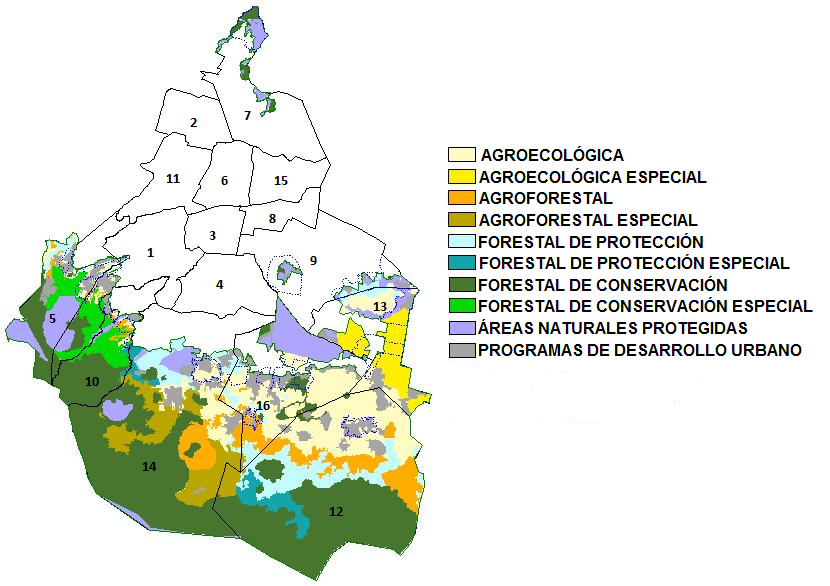
\includegraphics[width=100mm, scale=1]{ciudaddemexico}
  \caption{División política y uso de suelo en la Ciudad de México \citep{SEDEMA2016}}
  \label{ciudaddemexico}
\end{figure}

\newpage

El área de estudio contemplada en esta tesis se divide en 17 polígonos correspondientes a las 16 alcaldías de la Ciudad de México y el contorno de Ciudad Universitaria (campus principal de la UNAM) ubicada en la alcaldía Coyoacán, la cual es de especial interés debido a que alberga la Reserva Ecológica del Pedregal de San Ángel (REPSA).\\

La REPSA es una reserva natural de carácter urbano (no incluida en la categoría de suelo de conservación) protegida por la UNAM, lo cual garantiza un conocimiento ejemplar a través de las numerosas instituciones dedicadas a la investigación y divulgación científica. Su sustrato está conformado en su mayoría por roca basáltica la cual posee un alto valor biológico, ecológico y geomorfológico ya que permite recargar los mantos acuíferos, mantiene la humedad y la calidad del aire, y contribuye a amortiguar los cambios de temperatura en el microclima. La vegetación es de matorral xerófilo con marcada estacionalidad. Actualmente cuenta con una extensión de 237.33 hectáreas, que comprenden tres zonas núcleo y 13 zonas de amortiguamiento \citep{REPSA2019}.\\

En el Atlas de Riesgos de la REPSA \citep{AtlasREPSA} se cita la CL como una de las amenazas para los componentes biológicos del socioecosistema albergado por la REPSA y se menciona la necesidad de estudios en este sentido para la protección y conservación de la vida silvestre de Ciudad Universitaria.\\

La Ciudad de México está localizada en una zona sub-tropical donde las estaciones del año pueden ser separadas en tres periodos: Primavera Seca (PS) de abril a mayo, Temporada Lluviosa (TL) de junio a octubre e Invierno Seco (IS) de noviembre a marzo \citep{Jauregui2002}.\\

\subsection{Climatología de aerosol atmosférico y nubosidad}
\label{subsec:climatologia}

Para los fines de modelación de esta tesis resulta importante contar con la climatología de aerosol atmosférico y nubosidad en la Ciudad de México, como una referencia que permite realizar experimentos numéricos con condiciones cercanas a las reales.\\

\textbf{Aerosol atmosférico}

\cite{Carabali2017} realizaron la climatología de aerosol atmosférico para la Ciudad de México a partir de los datos obtenidos de 1999 a 2014 de la red AErosol RObotic NETwork (AERONET) para los periodos IS, PS y TL  (Tabla \ref{tab:climatologiaerosol}).\\

El AOD medido a 500 nm (AOD$_{500}$) provee una más robusta caracterización del AOD ya que a esa longitud de onda la absorción de vapor de agua y oxígeno es mínima \citep{Kanniah2009}. Por otro lado, el Parámetro de Angstrom calculado en el intervalo espectral 440-870 $(\alpha_{440-870})$ es el más adecuado para discriminar el tamaño de las partículas de aerosol atmosférico \citep{Kaskaoutis2007}.

\begin{table}[htb]
\centering
\caption{Climatología de aerosol atmosférico en la Ciudad de México \citep{Carabali2017}}
\label{tab:climatologiaerosol}
\resizebox{0.5\textwidth}{!}{%
\begin{tabular}{|c|c|c|}
\hline
\textbf{Periodo}        & \textbf{AOD$_{500}$} & \textbf{$\alpha_{440-870}$} \\ \hline
Invierno Seco (IS)      & 0.29         & 1.54           \\ \hline
Primavera Seca (PS)     & 0.33         & 1.49           \\ \hline
Temporada Lluviosa (TL) & 0.37         & 1.39           \\ \hline
\end{tabular}%
}
\end{table}

\newpage

\textbf{Nubosidad}

Aunque hasta la fecha no existe una climatología como tal de la nubosidad en la Ciudad de México, es posible inferir el tipo típico de nubes que se forman en cada uno de los periodos del año. Las nubes de interés para los experimentos numéricos de esta tesis son las nubes bajas y medias dada su cercanía en altitud con las fuentes artificiales de luz (Figura~\ref{nubes}).\\

A continuación se abordan las características de las nubes que forman parte del inventario del modelo \textit{SkyGlow} utilizado en este trabajo \citep{Cloudatlas1987}, \citep{Solano2015}.\\

\textit{\textbf{Altocumulus}}

\begin{itemize}

    \item Clasificación por altitud: nube media (3-5km)
    
    \item Formación: Generalmente a través de la condensación por ascenso de masas de aire húmedas
    
    \item Albedo espectral: 0.36 (350-800 nm)
    
\end{itemize}

\\

\textit{\textbf{Altostratus}}

\begin{itemize}

    \item Clasificación por altitud: nube media (3-5km)
    
    \item Formación: Asociadas a frentes (fríos, cálidos y ocluidos)
    
    \item Albedo espectral: 0.5 (350-800 nm)
    
\end{itemize}

\\

\textit{\textbf{Stratus}}

\begin{itemize}

    \item Clasificación por altitud: nube baja (700 m para este estudio)
    
    \item Formación: Condensación de masas de aire cálidas y húmedas en niveles bajos
    
    \item Albedo espectral: 0.5 (350-800 nm)
    
\end{itemize}

\\

\begin{figure}[htb]
  \centering
    \includegraphics[width=150mm, scale=1.5]{nubes}
  \caption{Nubes. A) Altocumulus, B) Altostratus, C) Stratus \citep{Metoffice2019}}
  \label{nubes}
\end{figure}

\newpage

\subsection{Consumo de energía eléctrica}
\label{subsec:consumoenergiaelectrica}

Con sólo 7\% de la población total de México, en la Ciudad de México se consume casi un tercio del petróleo demandado en el país y 6\% del total de la energía eléctrica \citep{SENER2013}. Las estadísticas muestran que del 100\% de energía eléctrica consumida en México, 30\% corresponde al sector residencial y de servicios públicos, sólo debajo del 52\% correspondiente a la industria \citep{Ramos2012}.\\

De acuerdo con el Sistema de Información Energética de la Secretaría de Energía, durante 2017 se consumieron en la Ciudad de México un total de 12,575,591 MW h$^{-1}$ de los cuales 2,938,559 MW h$^{-1}$ corresponden al sector residencial (23\%) de acuerdo con la Comisión Federal de Electricidad (Tabla \ref{tab:inventariocdmx}).\\

Es de interés conocer la relación entre el consumo de energía eléctrica y el cambio climático, lo cual es posible estimar a través de la emisión de Gases de Efecto Invernadero, más específicamente de CO$_{2}$ con el uso de la siguiente relación \citep{UTSEDEMA2018}: 

\begin{equation}
E_{CO_{2}} = W_{Elect}\: FE_{Elect}
\end{equation}

Donde $E_{CO_{2}}$ es la emisión en toneladas de CO$_{2}$ equivalente debida al consumo de energía eléctrica, $W_{Elect}$ es el consumo de energía eléctrica en MW h$^{-1}$ y $FE_{Elect}$ es el factor de consumo de energía eléctrica en toneladas de CO$_{2}$ equivalente por MW h$^{-1}$.\\

El factor de consumo de energía eléctrica se basa en el consumo total de combustible y la generación de electricidad neta entregada a la red. Varía cada año de acuerdo con la mezcla de combustibles empleados en la generación de electricidad distribuida por el Sistema Eléctrico Nacional, el cual está integrado por la Comisión Federal de Electricidad y productores independientes \citep{GEI2013}.\\

Considerando que el factor de consumo de energía eléctrica en 2017 fue 0.582 toneladas de CO$_{2}$ equivalente por MW h$^{-1}$ \citep{CRE2017}, se tiene que en 2017 se emitieron 7,318,993 toneladas de CO$_{2}$ por consumo de energía eléctrica en la Ciudad de México (6\% del total de las emisiones nacionales de CO$_{2}$ por consumo de energía eléctrica).\\

\subsection{Inventario de Alumbrado Público de la Ciudad de México}

Gracias a los datos brindados por las oficinas de transparencia de cada una de las alcaldías de la Ciudad de México y la Agencia de Gestión Urbana a través del Instituto de Transparencia, Acceso a la Información Pública, Protección de Datos Personales y Rendición de Cuentas de la Ciudad de México se construyó el \textbf{Inventario de Alumbrado Público de la Ciudad de México} (Tabla \ref{tab:inventariocdmx}).\\

Los datos de consumo de energía eléctrica por entidad federativa se obtuvieron a través del Sistema de Información Energética de la Secretaría de Energía (\url{sie.energia.gob.mx}}) y los datos de consumo de energía eléctrica por municipio producidos por la Comisión Federal de Electricidad se obtuvieron a través de la Plataforma Datos Abiertos del Gobierno de México (\url{datos.gob.mx}}).\\

\newpage

\begin{landscape}
\begin{table}[]
\centering
\caption{Inventario de Alumbrado Público de la Ciudad de México}
\label{tab:inventariocdmx}
\resizebox{1.4\textwidth}{!}{%
\begin{tabular}{llcccllcccc}
\hline
\multicolumn{1}{|c|}{\textbf{$\#$}} & \multicolumn{1}{c|}{\textbf{Alcaldía}} & \multicolumn{1}{l|}{\textbf{Extensión (km$^{2}$)}} & \multicolumn{1}{c|}{\textbf{\begin{tabular}[c]{@{}c@{}}Población\\ (número de habitantes)\end{tabular}}} & \multicolumn{1}{c|}{\textbf{Halogenuros metálicos ($\%$)}} & \multicolumn{1}{c|}{\textbf{LED ($\%$)}} & \multicolumn{1}{c|}{\textbf{\begin{tabular}[c]{@{}c@{}}Vapor de sodio de\\ alta presión ($\%$)\end{tabular}}} & \multicolumn{1}{c|}{\textbf{\begin{tabular}[c]{@{}c@{}}Número de luminarias\\ (vías primarias)\end{tabular}}} & \multicolumn{1}{c|}{\textbf{\begin{tabular}[c]{@{}c@{}}Número de luminarias\\ (vías secundarias)\end{tabular}}} & \multicolumn{1}{c|}{\textbf{\begin{tabular}[c]{@{}c@{}}Número de luminarias\\ (totales)\end{tabular}}} & \multicolumn{1}{c|}{\textbf{\begin{tabular}[c]{@{}c@{}}Consumo de energía eléctrica\\ sector residencial (MW h$^{-1}$)\end{tabular}}} \\ \hline
 &  & \multicolumn{1}{l}{} & \multicolumn{1}{l}{} & \multicolumn{1}{l}{} &  &  & \multicolumn{1}{l}{} & \multicolumn{1}{l}{} & \multicolumn{1}{l}{} & \multicolumn{1}{l}{} \\ \hline
\multicolumn{1}{|l|}{1} & \multicolumn{1}{l|}{Álvaro Obregón} & \multicolumn{1}{c|}{96.17} & \multicolumn{1}{c|}{749,982} & \multicolumn{1}{c|}{62} & \multicolumn{1}{c|}{} & \multicolumn{1}{c|}{38} & \multicolumn{1}{c|}{9,911} & \multicolumn{1}{c|}{71,397} & \multicolumn{1}{c|}{40,835} & \multicolumn{1}{c|}{210,903} \\ \hline
\multicolumn{1}{|l|}{2} & \multicolumn{1}{l|}{Azcapotzalco} & \multicolumn{1}{c|}{33.6} & \multicolumn{1}{c|}{400,161} & \multicolumn{1}{c|}{100} & \multicolumn{1}{l|}{} & \multicolumn{1}{c|}{} & \multicolumn{1}{c|}{5,009} & \multicolumn{1}{c|}{22,527} & \multicolumn{1}{c|}{27,536} & \multicolumn{1}{c|}{168,877} \\ \hline
\multicolumn{1}{|l|}{3} & \multicolumn{1}{l|}{Benito Juárez} & \multicolumn{1}{c|}{26.63} & \multicolumn{1}{c|}{417,416} & \multicolumn{1}{c|}{93} & \multicolumn{1}{c|}{7} & \multicolumn{1}{l|}{} & \multicolumn{1}{c|}{8,862} & \multicolumn{1}{c|}{27,550} & \multicolumn{1}{c|}{36,412} & \multicolumn{1}{c|}{234,458} \\ \hline
\multicolumn{1}{|l|}{4} & \multicolumn{1}{l|}{Coyoacán} & \multicolumn{1}{c|}{54.12} & \multicolumn{1}{c|}{608,479} & \multicolumn{1}{c|}{100} & \multicolumn{1}{l|}{} & \multicolumn{1}{l|}{} & \multicolumn{1}{c|}{6,463} & \multicolumn{1}{c|}{36,856} & \multicolumn{1}{c|}{43,319} & \multicolumn{1}{c|}{230,390} \\ \hline
\multicolumn{1}{|l|}{5} & \multicolumn{1}{l|}{Cuajimalpa de Morelos} & \multicolumn{1}{c|}{80.95} & \multicolumn{1}{c|}{199,224} & \multicolumn{1}{c|}{90} & \multicolumn{1}{l|}{} & \multicolumn{1}{c|}{10} & \multicolumn{1}{c|}{1,147} & \multicolumn{1}{c|}{13,186} & \multicolumn{1}{c|}{14,333} & \multicolumn{1}{c|}{72,127} \\ \hline
\multicolumn{1}{|l|}{6} & \multicolumn{1}{l|}{Cuauhtémoc} & \multicolumn{1}{c|}{32.44} & \multicolumn{1}{c|}{532,553} & \multicolumn{1}{c|}{100} & \multicolumn{1}{l|}{} & \multicolumn{1}{l|}{} & \multicolumn{1}{c|}{12,574} & \multicolumn{1}{c|}{26,938} & \multicolumn{1}{c|}{39,512} & \multicolumn{1}{c|}{286,460} \\ \hline
\multicolumn{1}{|l|}{7} & \multicolumn{1}{l|}{Gustavo A. Madero} & \multicolumn{1}{c|}{94.07} & \multicolumn{1}{c|}{1,164,477} & \multicolumn{1}{c|}{99} & \multicolumn{1}{c|}{1} & \multicolumn{1}{l|}{} & \multicolumn{1}{c|}{13,778} & \multicolumn{1}{c|}{46,362} & \multicolumn{1}{c|}{60,140} & \multicolumn{1}{c|}{415,940} \\ \hline
\multicolumn{1}{|l|}{8} & \multicolumn{1}{l|}{Iztacalco} & \multicolumn{1}{c|}{23.3} & \multicolumn{1}{c|}{390,348} & \multicolumn{1}{c|}{100} & \multicolumn{1}{l|}{} & \multicolumn{1}{l|}{} & \multicolumn{1}{c|}{6,056} & \multicolumn{1}{c|}{23,050} & \multicolumn{1}{c|}{29,106} & \multicolumn{1}{c|}{145,105} \\ \hline
\multicolumn{1}{|l|}{9} & \multicolumn{1}{l|}{Iztapalapa} & \multicolumn{1}{c|}{116.1} & \multicolumn{1}{c|}{1,827,868} & \multicolumn{1}{c|}{100} & \multicolumn{1}{l|}{} & \multicolumn{1}{l|}{} & \multicolumn{1}{c|}{12,700} & \multicolumn{1}{c|}{91,148} & \multicolumn{1}{c|}{103,848} & \multicolumn{1}{c|}{530,447} \\ \hline
\multicolumn{1}{|l|}{10} & \multicolumn{1}{l|}{Magdalena Contreras} & \multicolumn{1}{c|}{63.61} & \multicolumn{1}{c|}{243,886} & \multicolumn{1}{c|}{95} & \multicolumn{1}{c|}{5} & \multicolumn{1}{l|}{} & \multicolumn{1}{c|}{999} & \multicolumn{1}{c|}{9,200} & \multicolumn{1}{c|}{10,199} & \multicolumn{1}{c|}{44,762} \\ \hline
\multicolumn{1}{|l|}{11} & \multicolumn{1}{l|}{Miguel Hidalgo} & \multicolumn{1}{c|}{46.99} & \multicolumn{1}{c|}{364,439} & \multicolumn{1}{c|}{95} & \multicolumn{1}{c|}{5} & \multicolumn{1}{l|}{} & \multicolumn{1}{c|}{10,920} & \multicolumn{1}{c|}{30,838} & \multicolumn{1}{c|}{41,758} & \multicolumn{1}{c|}{185,013} \\ \hline
\multicolumn{1}{|l|}{12} & \multicolumn{1}{l|}{Milpa Alta} & \multicolumn{1}{c|}{228.4} & \multicolumn{1}{c|}{137,927} & \multicolumn{1}{c|}{100} & \multicolumn{1}{l|}{} & \multicolumn{1}{l|}{} & \multicolumn{1}{c|}{268} & \multicolumn{1}{c|}{10,226} & \multicolumn{1}{c|}{10,494} & \multicolumn{1}{c|}{20,645} \\ \hline
\multicolumn{1}{|l|}{13} & \multicolumn{1}{l|}{Tláhuac} & \multicolumn{1}{c|}{83.45} & \multicolumn{1}{c|}{361,593} & \multicolumn{1}{c|}{97} & \multicolumn{1}{c|}{3} & \multicolumn{1}{l|}{} & \multicolumn{1}{c|}{2,030} & \multicolumn{1}{c|}{18,389} & \multicolumn{1}{c|}{20,419} & \multicolumn{1}{c|}{90,984} \\ \hline
\multicolumn{1}{|l|}{14} & \multicolumn{1}{l|}{Tlalpan} & \multicolumn{1}{c|}{312} & \multicolumn{1}{c|}{677,104} & \multicolumn{1}{c|}{100} & \multicolumn{1}{l|}{} & \multicolumn{1}{l|}{} & \multicolumn{1}{c|}{5,313} & \multicolumn{1}{c|}{3,321} & \multicolumn{1}{c|}{8,634} & \multicolumn{1}{c|}{21,367} \\ \hline
\multicolumn{1}{|l|}{15} & \multicolumn{1}{l|}{Venustiano Carranza} & \multicolumn{1}{c|}{33.42} & \multicolumn{1}{c|}{427,263} & \multicolumn{1}{c|}{100} & \multicolumn{1}{l|}{} & \multicolumn{1}{l|}{} & \multicolumn{1}{c|}{9,970} & \multicolumn{1}{c|}{28,481} & \multicolumn{1}{c|}{38,451} & \multicolumn{1}{c|}{175,050} \\ \hline
\multicolumn{1}{|l|}{16} & \multicolumn{1}{l|}{Xochimilco} & \multicolumn{1}{c|}{122} & \multicolumn{1}{c|}{415,933} & \multicolumn{1}{c|}{95} & \multicolumn{1}{c|}{5} & \multicolumn{1}{l|}{} & \multicolumn{1}{c|}{1,488} & \multicolumn{1}{c|}{22,459} & \multicolumn{1}{c|}{23,947} & \multicolumn{1}{c|}{106,031} \\ \hline
 &  & \multicolumn{1}{l}{} & \multicolumn{1}{l}{} & \multicolumn{1}{l}{} &  &  & \multicolumn{1}{l}{} & \multicolumn{1}{l}{} & \multicolumn{1}{l}{} & \multicolumn{1}{l}{} \\ \cline{7-11} 
 &  & \multicolumn{1}{l}{} & \multicolumn{1}{l}{} & \multicolumn{1}{l}{} & \multicolumn{1}{l|}{} & \multicolumn{1}{c|}{\textbf{Total}} & \multicolumn{1}{c|}{107,488} & \multicolumn{1}{c|}{481,928} & \multicolumn{1}{c|}{589,416} & \multicolumn{1}{c|}{2,938,559} \\ \cline{7-11} 
\end{tabular}
}
\end{table}
\end{landscape}

\section{Hipótesis}

\vspace{5mm}

La cantidad, distribución y características de luz artificial producida por el alumbrado público da origen al brillo del cielo nocturno, que en mayor o menor medida, genera contaminación lumínica en las alcaldías de la Ciudad de México.\\

De manera general se considera que existe contaminación lumínica cuando los valores de radiancia son mayores al máximo valor natural registrado, es decir \textbf{10$^{-4}$ W sr$^{-1}$  m$^{-2}$} (véase \textbf{\autoref{subsec:componentesbrillocielo}}).\\

\section{Objetivos}

\vspace{5mm}

\subsection{Generales}

\vspace{5mm}

\begin{itemize}

	\item Estimar los niveles de contaminación lumínica en la Ciudad de México 

    \item Reproducir el modelo \textit{SkyGlow} para el caso de la Ciudad de México
    
    \item Generar un antecedente para la campaña de validación del modelo \textit{SkyGlow} en la Ciudad de México
    
\end{itemize}

\vspace{5mm}

\subsection{Particulares}

\begin{itemize}

    \item Elaborar el \textbf{Inventario de Alumbrado Público de la Ciudad de México}
    
    \item Generar el \textbf{Mapa Teórico de Contaminación Lumínica de la Ciudad de México} con salidas del modelo \textit{SkyGlow} 
    
    \item Estimar la tendencia de los valores de radiancia en las alcaldías de la Ciudad de México
    
    \item Construir mediante experimentos numéricos con el modelo \textit{SkyGlow} diferentes escenarios del brillo del cielo nocturno tomando en cuenta diferentes posiciones del observador y condiciones atmosféricas
    
    \item Inferir la influencia del aerosol atmosférico  y la nubosidad en el brillo del cielo nocturno de la Ciudad de México a partir del objetivo anterior
    
    
\end{itemize}
	
	\chapter{Metodología}
\label{chap:metodologia}

En este capítulo se describen las bases teóricas y técnicas del modelo de distribución de la luz en la atmósfera \textit{SkyGlow} desarrollado por \cite{Kocifaj2007}, además del software \textit{Radiance Light Trends} desarrollado por \cite{RLT2019} que permite analizar datos de radiancia medidos por el sensor \textit{Visible Infrared Imaging Radiometer Suite} (VIIRS) a bordo del satélite \textit{Suomi National Polar-orbiting Partnership}.\\

Advertencia: la distribución de radiancia teórica generada por el modelo \textit{SkyGlow} se construye considerando un observador en superficie por lo que, al comparar los valores de radiancia teóricos del modelo con los generados por el VIIRS, no se pretende validar el modelo, sino estimar la tendencia de los valores de radiancia para el área de interés.\\

En el \textbf{\autoref{chap:recomendaciones}} se presentan propuestas para validar el modelo \textit{SkyGlow} para la Ciudad de México.\\ 

\section{El modelo \textit{SkyGlow}}


\textit{SkyGlow} es un modelo teórico escalable que permite simular el comportamiento angular de la radiancia en el cielo durante la noche en una región específica o integrada del EE. No considera restricciones en el número de fuentes de luz ni en la distribución espacial de las mismas en la vecindad del punto de medición, por lo que la distancia y el ángulo acimutal de las fuentes de luz son configurables. El modelo es aplicable para fuentes de luz con dimensiones finitas reales con propiedades radiativas espectrales y angulares definidas \citep{Kocifaj2007}.\\ 

La influencia de la atmósfera en la modulación de la radiación es formulada en términos de propiedades ópticas de las moléculas de aire y aerosol atmosférico. La reflectancia espectral y la altitud de las capas de nubes son los principales factores tomados en cuenta para la modelación de condiciones de nubosidad \citep{Kocifaj2007}, \citep{Solano2014}.\\ 

Las ecuaciones derivadas son traducidas en código numéricamente rápido, lo que es deseable para la realización de experimentos numéricos que incluyen una malla con gran número de puntos (dominio geográfico grande con alta resolución espacial) \citep{Kocifaj2007}, \citep{Linares2018}.\\

\subsection{Datos de entrada}

\textbf{Definición del dominio}

El área de la superficie de estudio (forma y tamaño) es definida a través de vértices coordenados (latitud y longitud). \textit{Para este estudio}: polígonos de cada una de las 16 alcaldías de la Ciudad de México y de la REPSA (Figura~\ref{ciudaddemexicomodelo}).

\newpage

\begin{figure}
  \centering
    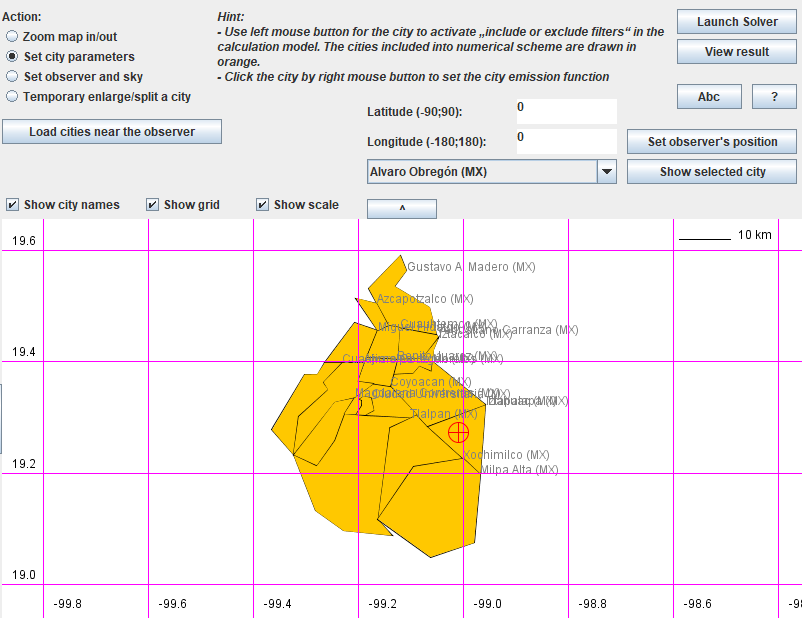
\includegraphics[width=0.6\textwidth]{ciudaddemexicomodelo}
  \caption{Intefaz gráfica del modelo \textit{SkyGlow}}
  \label{ciudaddemexicomodelo}
\end{figure}

\textbf{Inventario de fuentes de luz}

El modelo calcula la emisión total de las fuentes de luz con base en la población (típicamente 750 lm por habitante) y su dependencia espectral \textit{Para este estudio}: datos del \textbf{Inventario de Alumbrado Público de la Ciudad de México} (Tabla \ref{tab:inventariocdmx}).\\

\textbf{Variables del caso de estudio}

Una vez que el escenario está definido, el modelo requiere de parámetros específicos del experimento numérico que se desarrollará:

\begin{itemize}

    \item Rango de longitud de onda: la máxima y mínima longitud de onda a estudiar. \textit{Para este estudio}: rango visible del EE dividido en 40 ventanas de 10 nm, con el fin  de estimar el efecto de la dependencia espectral de las fuentes de luz reportadas en el \textbf{Inventario de Alumbrado Público de la Ciudad de México}.
    
    \item Aerosol atmosférico: véase la \textbf{\autoref{subsubsec:propiedadesopticasaerosol}}. \textit{Para este estudio}: los experimentos numéricos se realizaron considerando la climatología descrita en la \textbf{\autoref{subsec:climatologia}}. Para condiciones de fondo promedio (FP) se considera el AOD = 0.1, Parámetro de Angstrom $\alpha$ = 1.3, ASY = 0.6 y Albedo de Dispersión Simple SSA = 0.85; Para especies carbonosas (EC, carbón elemental producto de la combustión incompleta de combustibles fósiles y carbón orgánico) AOD = 0.1, $\alpha$ = 1.3, ASY = 0.3, SSA = 0.3. (Todos los parámetros constantes a lo largo del espectro estudiado) \citep{Penner1998}, \citep{Schmidt2010}.
    
    \item Nubosidad: altura y albedo espectral de la capa de nube. \textit{Para este estudio}: véase la \textbf{\autoref{subsec:climatologia}}
    
    \item Posición del observador: en coordenadas (latitud y longitud) 
    
\end{itemize}

\subsection{Bases teóricas del modelo}

La intensidad de la luz que crea el patrón del brillo del cielo en un volumen atmosférico elemental es la suma de todas las intensidades de todos los rayos emitidos de diferentes áreas en diferentes ángulos cenitales. \cite{Kocifaj2007} expresa la radiancia espectral (W sr$^{-1}$  m$^{-2}$ nm$^{-1}$) del cielo despejado como:

\begin{equation}\label{eq:2.1}
I_{\lambda}(z, \phi) = \frac{A_{0}\, S_{\lambda}}{cos\,z} \int_{h=0}^{h} B_{\lambda}(Q, q, z') \: \Gamma_{\lambda} \:(h, z, \phi, z', \phi') \: T_{\lambda}(h, z, \phi) \: \frac{cos^{2}z'}{h^{2}} dh
\end{equation}

Donde $\lambda$ es la longitud de onda a la que se emite la luz, $z'$ y $\phi'$ son el ángulo cenital y acimutal de la luz emitida respectivamente, mientras que $z$ y $\phi$ caracterizan la posición del elemento de cielo observado y h es su altura con respecto al observador P (Figura~\ref{geometriamodelo}).\\

El primer término de la izquierda de la ecuación captura la emisión de las fuentes de luz (no dependen del observador) donde $A_{0}$ es un elemento de superficie de una fuente de luz que radia en todas direcciones y $S_{\lambda}$ es la potencia emitida por elemento de superficie $A_{0}$ de la fuente radiante (W m$^{-2}$ nm$^{-1}$).\\


\begin{figure}[htb]
  \centering
    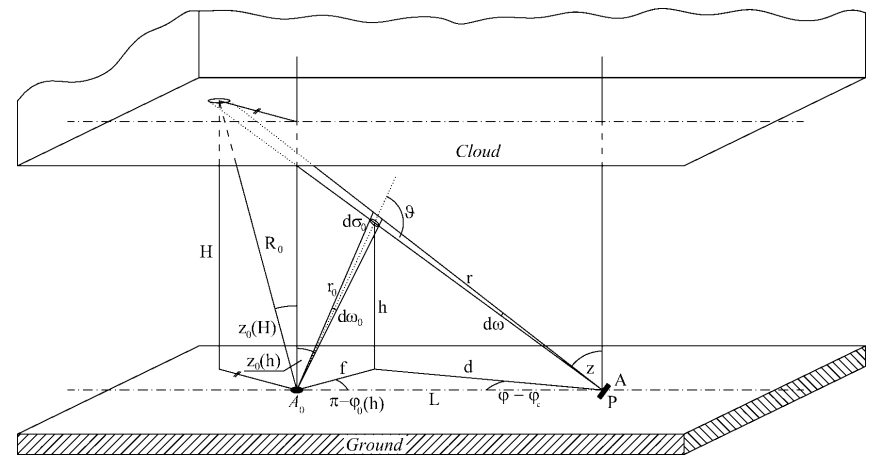
\includegraphics[width=1\textwidth]{geometriamodelo}
  \caption{Geometría del modelo \citep{Kocifaj2007}}
  \label{geometriamodelo}
\end{figure}


Los procesos capturados por los términos dentro de la integral se desarrollan en la atmósfera (por ello están integrados desde la superficie hasta la altura h). $B$ es la CEF abordada en la \textbf{\autoref{subsec:climatologia}}; esta función determina el comportamiento angular de la radiación emitida por las fuentes de luz. La aproximación semi-empírica a la CEF (Garstang Emission Function, GEF) que \cite{Garstang1986} desarrolló es:

\begin{equation}
B(Q, q, z') = 2Q(1-q) cos \, z' + 0.554q \,z'^{4}
\end{equation}

Donde $Q$ es la fracción de la luz que es reflejada isotrópicamente desde la superficie y $q$ es la fracción radiada directamente hacia arriba, con respecto al ángulo cenital $z'$. La \textbf{Tabla \ref{tab:valoresdeq}} muestra los valores de q utilizados para este estudio.\\


\begin{table}[htb]
\centering
\caption{Fracción $q$ radiada directamente hacia arriba en el ángulo cenital $z'$ \citep{Kocifaj2007}}
\label{tab:valoresdeq}
\resizebox{0.5\textwidth}{!}{%
\begin{tabular}{|c|c|c|c|c|c|c|c|c|c|c|}
\hline
\textbf{z'} & 0 & 10 & 20 & 30 & 40 & 50 & 60 & 70 & 80 & 90 \\ \hline
\textbf{q} & 1 & 0.95 & 0.8 & 0.7 & 0.6 & 0.5 & 0.4 & 0.3 & 0.15 & 0 \\ \hline
\end{tabular}%
}
\end{table}

Resulta importante mencionar que \cite{Kocifaj2016} señalan la falta de validez de la GEF en algunos casos. La GEF sobrestima las emisiones en ángulos cenitales bajos debido a que estas son fácilmente suprimidas por obstáculos.\\

 Sin embargo, ya que el modelo \textit{SkyGlow} está basado en el Método de Órdenes de Dispersión Sucesivos (MODS)\footnote{El MODS modela la intensidad de una señal dispersada a través de una expansión en serie de varios órdenes sucesivos. \textit{SkyGlow} únicamente toma el primer orden de la serie (dispersión simple) \citep{USENERGY2017}} con fuentes de tamaño finito, las deficiencias de la GEF no resultan críticas \citep{USENERGY2017}.\\

Continuando con el análisis de la ecuación \ref{eq:2.1}, $\Gamma$ es una función que caracteriza la distribución angular de la luz dispersada de un volumen elemental de la atmósfera en una altura $h$. Se calcula como el producto del coeficiente de dispersión y la función de fase de dispersión (véase la \textbf{\autoref{subsubsec:propiedadesopticasaerosol}}). $\Gamma$ varía con el ángulo de dispersión $\vartheta$ en $h$, que a su vez depende de la dirección de observación, la dirección de los rayos emitidos y la distancia $L$ entre la fuente de luz y el observador:

\begin{equation}
cos \, \vartheta_{h} = \frac{1}{2} \left(\frac{L^{2}}{h^{2}} \: cos \, z \: cos \, z' - \frac{cos \, z'}{cos \, z}- \frac{cos \, z}{cos \, z'}\right)
\end{equation}


Por último, $T$ es una función que caracteriza la atenuación atmosférica en términos del AOD:

\begin{equation}
T_{\lambda}(h, z, \phi) = t_{\lambda}(h,z) \, t_{\lambda}(h, z')
\end{equation}

Si la radiancia espectral $I_{\lambda}(z, \phi)$ es conocida, entonces la irradiancia espectral difusa en una superficie horizontal $D_{\lambda}$ puede ser calculada \citep{Kocifaj2014} como: 

\begin{equation} \label{eq:2.5}
D_{\lambda} = \int_{z = 0}^{z =\pi/2} \int_{\phi = 0}^{\phi = 2\pi} I_{\lambda} (z, \phi) \: sen \,z \: dz \: d\phi
\end{equation}

Para el caso en que se considera cielo nublado, se suma a la ecuación \ref{eq:2.1} el término de la interacción del flujo de luz con una capa nubosa a una altura $H$:

\begin{equation} \label{eq:2.6}
I_{\lambda, Nube}(z, \phi) = S_{\lambda} \: \frac{A_{0} \, \rho_{\lambda}(z'_{H}, z, \vartheta_{H})}{\pi H^{2}} \: B_{\lambda}(Q, q, z'_{H}) \: T_{\lambda}(H, z, \phi) \: cos^{4} \, z'_{H}
\end{equation}

Donde $\rho$ es la reflectancia espectral de la nube, $z'_{H}$ es el ángulo cenital de la luz emitida con respecto al elemento de área radiante de la nube y $\vartheta_{H}$ es el ángulo de dispersión en $H$. Sumando la ecuación \ref{eq:2.1} y \ref{eq:2.6} se obtiene la expresión para la radiancia espectral total con cielo nublado $I_{\lambda, Total}(z, \phi)$.

\newpage

Considerando que el punto del observador está rodeado de $N$ fuentes de luz, donde la características radiativas de la $i$ésima fuente son $S_{i}$, $Q_{i}$, $q_{i}$ y la distancia y el ángulo acimutal de la $i$ésima fuente son $L_{i}$ y $\phi_{i}$ respectivamente. La cantidad total de la intensidad de la luz dispersada es calculada como la suma de todas las fuentes: 

\begin{equation}
J(z, \phi) = \sum_{i=1}^{N} \int_{\lambda_{1}}^{\lambda_{2}} I_{\lambda, i}(z, \phi)  \: d\lambda
\end{equation}

\subsection{Visualización de datos de salida}

Las salidas del modelo son:

\begin{itemize}


	\item irradiancia espectral (W m$^{-2}$) difusa en una superficie horizontal

	\item radiancia (W m$^{-2}$ sr $^{-1}$) en $z$ ($0\grad - 85\grad$), $\;$  $\phi$ ($0\grad - 360\grad$)

    
\end{itemize}



\textbf{Gráficas tipo \textit{all-sky}}\\

La distribución de la radiancia integral en el cielo se visualiza con gráficas polares del logaritmo de las salidas de radiancia del modelo (Figura~\ref{graficapolar}). Estas gráficas se interpretan como la radiancia que llega a un observador desde todas las partes del cielo (180\grad), por lo que son denominadas gráficas tipo \textit{all-sky}. El ángulo a lo largo del círculo representa el ángulo acimutal $\phi$ mientras que el ángulo cenital $z$ es medido desde el centro hasta el margen de la gráfica.\\

El código fue desarrollado por el Dr. Miroslav Kocifaj de la Academia Eslovaca de Ciencias en gnuplot y está integrado en el modelo \textit{SkyGlow}.\\


\begin{figure}[htb]
  \centering
    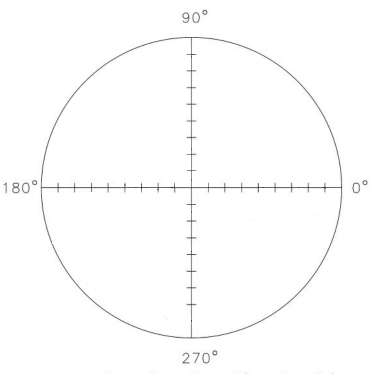
\includegraphics[width=0.3\textwidth]{graficapolar}
  \caption{Gráfica polar}
  \label{graficapolar}
\end{figure}\\


\textbf{Mapa coroplético}}\\

El \textbf{Mapa Teórico de Contaminación Lumínica de la Ciudad de México} (Mapa CL-CDMX) es un mapa coroplético de irradiancia espectral difusa en una superficie horizontal calculada con \textit{SkyGlow} con condiciones de FP. El código desarrollado en Julia se presenta en el \textbf{\autoref{chap:anexos}}. Los polígonos de sectores de la Ciudad de México se obtuvieron de la página de Datos Abiertos Ciudad de México (\url{datos.cdmx.gob.mx}}) y se tradujeron al formato TopoJSON con la biblioteca de software GDAL.

\newpage

\section{El software \textit{Radiance Light Trends}}

\textit{Radiance Light Trends} es una aplicación web (\url{lighttrends.lightpollutionmap.info}}) que permite analizar tendencias mundiales de radiancia promedio desde 2013 hasta la fecha con datos satelitales nocturnos de la Banda Día/Noche (DNB, por sus siglas en inglés) del VIIRS, disponibles en la página \textit{National Centers for Environmental Information} (\url{https://ngdc.noaa.gov/}}) de la \textit{National Oceanic and Atmospheric Administration} (NOAA).\\

\subsection{Especificaciones}

La DNB está especialmente diseñada para observar la luz artificial a escala mundial. Escanea una región alrededor de la 1:30 am en un rango espectral de 500-900 nm con una resolución espacial de 0.5 km$^2$ \citep{Elvidge2017}.\\

\subsection{Consideraciones}

Las imágenes captadas por la DNB son filtradas para reducir ruido de fondo, contaminación de radiancia debida a la luz solar y lunar y cobertura nubosa. Sin embargo, pueden observarse variaciones en corto plazo (meses) debido al ángulo de las imágenes con que se hacen las composiciones mensuales, incendios, fuegos artificiales y bengalas. Debido a esto, resulta recomendable analizar los datos de la DNB en tendencias a largo plazo (anuales) para centrarse en las variables de interés: la variación de la radiancia debido al cambio de los sistemas de iluminación (número, fuente y distribución espacial) \citep{Coesfeld2018}, \citep{Elvidge2017}.\\

\subsection{Productos}

La aplicación calcula para cada polígono de cada alcaldía de la Ciudad de México la radiancia promedio anual y le ajusta una línea de tendencia exponencial y una máscara cuando la región es mayor a 100 km$^2$. Además, la interfaz gráfica de la aplicación permite visualizar una composición de imágenes de la DNB de radiancia promedio para el 2016 (Figura~\ref{radiancetrends}) en la que, cualitativamente, las regiones más claras indican valores más altos de radiancia.

\begin{figure}[htb]
  \centering
    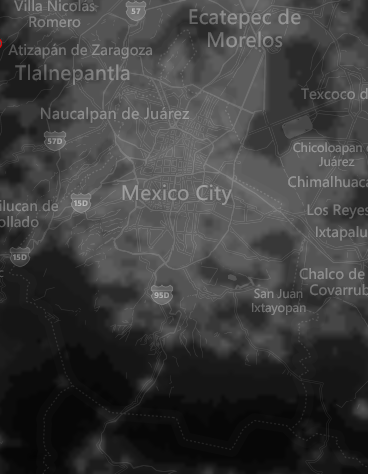
\includegraphics[width=0.3\textwidth]{RadianceTrends}
  \caption{Composición de imágenes satelitales de radiancia en la Ciudad de México (imagen y datos procesados por la NOAA, bajo los términos de uso de Microsoft\textregistered \: Bing\textsuperscript{TM} \: Maps Platform)}
  \label{radiancetrends}
\end{figure}
	
	\chapter{Resultados y discusión}

La composición de imágenes satelitales de radiancia en la Ciudad de México (Figura~\ref{radiancetrends}) muestra cualitativamente que los niveles más altos de radiancia promedio se encuentran en la fracción norte-centro de la ciudad, lo que naturalmente, coincide con los asentamientos urbanos. Dada esta distribución, se considera que un observador está <<dentro de la ciudad>> cuando se encuentra en alguno de los Sectores Urbanos mostrados en el Mapa CL-CDMX y <<fuera de la ciudad>> cuando está fuera de ellos, lo que corresponde con suelo de conservación. 

\section{Tendencias de radiancia promedio en las alcaldías de la Ciudad de México}
\label{subsec:tendenciasradiancia}

Por efectos de representatividad se selecionaron las siguientes figuras elaboradas con el software \textit{Radiance Light Trends} que muestran las tendencias de radiancia promedio en la alcaldía Gustavo A. Madero (GAM, densamente poblada), Milpa Alta (MA, menos poblada, con mayoría de territorio en suelo de conservación) y en el polígono de CU que contiene la REPSA. El resto de las tendencias por alcaldía se encuentran en el \textbf{\autoref{chap:anexos}}.

\begin{figure}[htb]
  \centering
    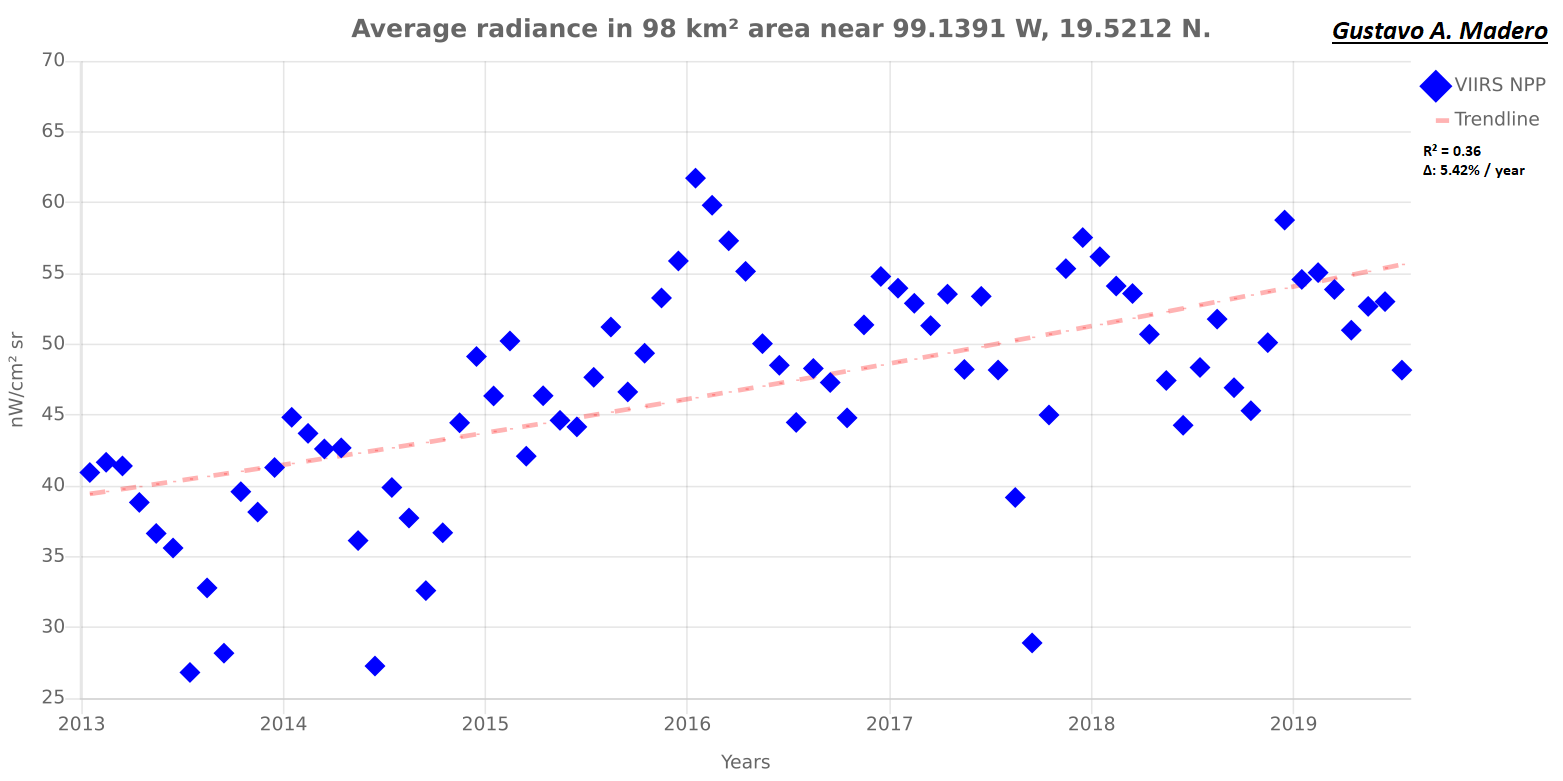
\includegraphics[width=1\textwidth]{GAM}
  \caption{Tendencia de radiancia promedio para la alcaldía GAM}
  \label{radiancetrendsgam}
\end{figure}

\newpage


\begin{figure}[H]
  \centering
    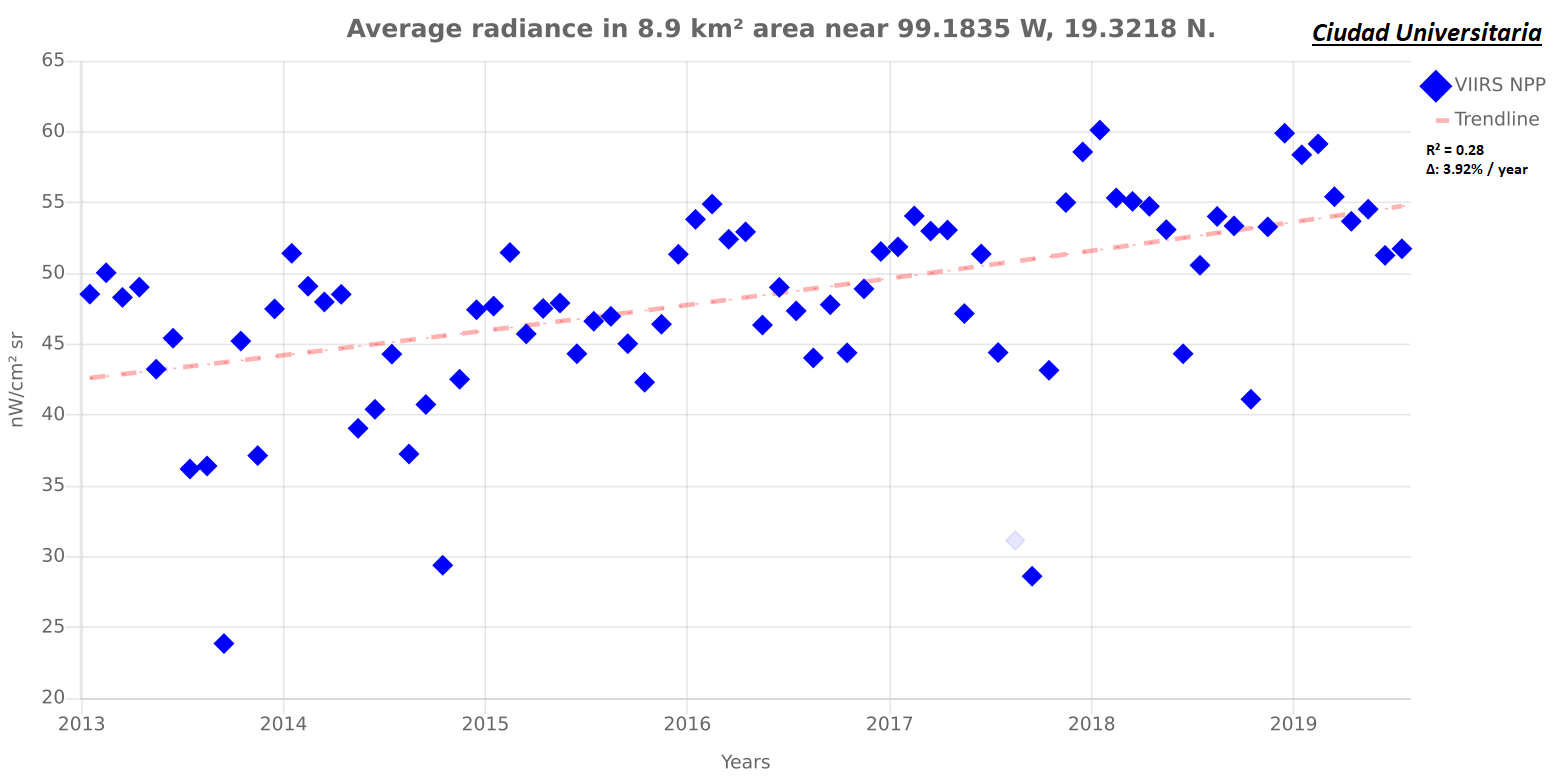
\includegraphics[width=1\textwidth]{CU}
  \caption{Tendencia de radiancia promedio para CU}
  \label{radiancetrendscu}
\vspace{20mm} 
    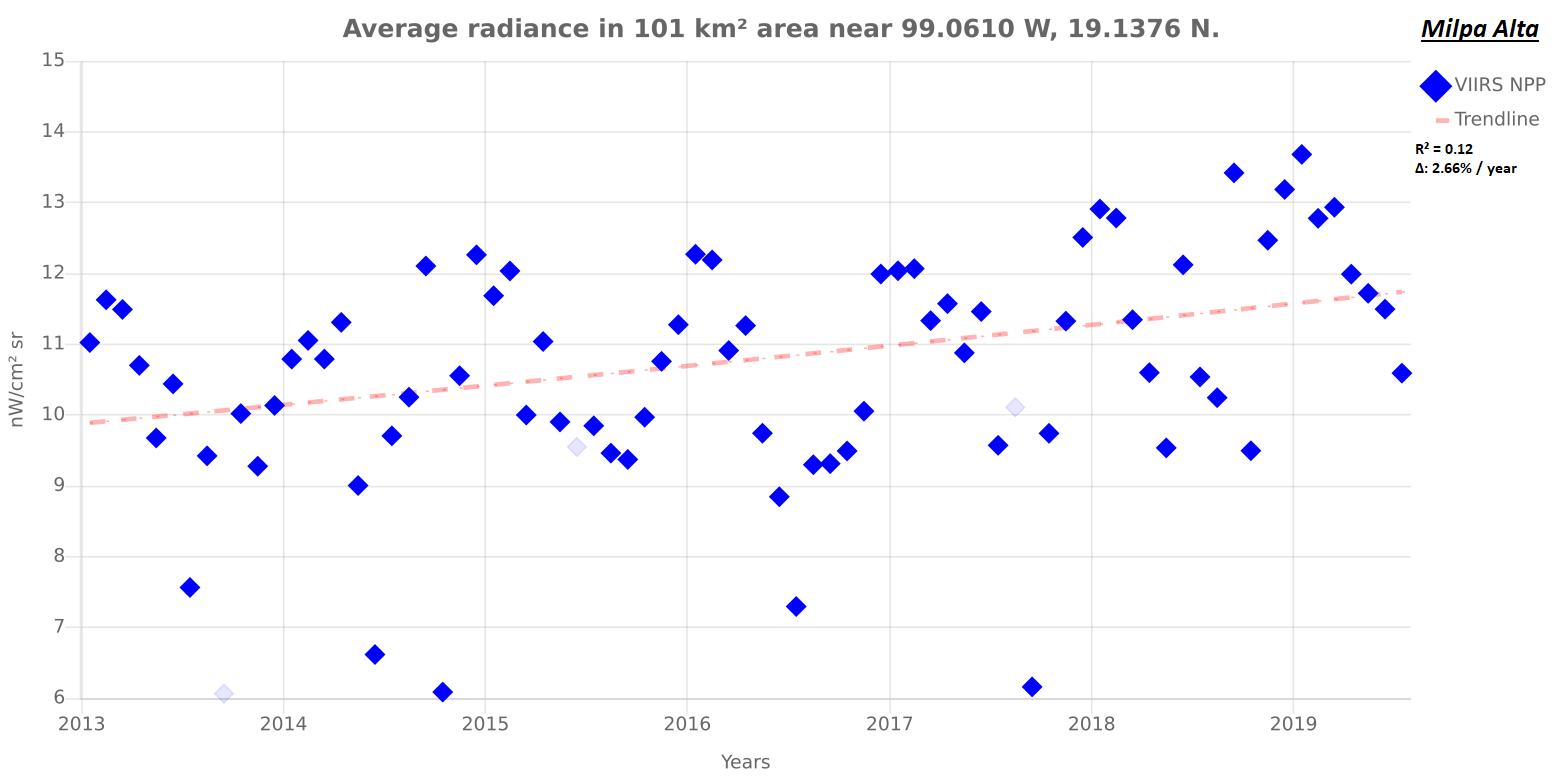
\includegraphics[width=1\textwidth]{MA}
  \caption{Tendencia de radiancia promedio para la alcaldía MA}
  \label{radiancetrendsma}
\end{figure}
\blindtext

\newpage

Como se muestra en el \textbf{Inventario de Alumbrado Público de la Ciudad de México}, hoy en día el principal tipo de fuente de luz del alumbrado público de la Ciudad de México es la lámpara de halogenuros metálicos. Sin embargo, de manera histórica, el número de luminarias y sus características han ido cambiando, lo que sumado a la fluctuación de  las luminarias residenciales y privadas ha tenido efecto en las tendencias de radiancia en las diferentes alcaldías de la ciudad.\\

De acuerdo con \cite{Universal2017} durante 2015 se destinaron 2600 millones de pesos mexicanos para el programa <<Iluminemos Tu Ciudad>>, que llevó a cabo el cambio de luminarias en vías primarias y secundarias de la Ciudad de México. Se menciona este hecho como la actualización de una <<tecnología de la década de 1990 por una más limpia>>.\\

La fuente de luz de las antiguas luminarias mencionadas era de halogenuros metálicos con un tubo de descarga de cuarzo mientras que las nuevas también tienen fuente de de halogenuros metálicos pero con la diferencia que el tubo de descarga es de cerámica, lo que algunos fabricantes mencionan 10-20\% más eficiente \citep{EMB2007}.\\

En pocas palabras, la dependencia espectral del alumbrado de la ciudad no cambió durante la aplicación del programa. En este punto es importante mencionar que la cualidad de <<limpia>> a la que los encargados del programa se refieren, no tiene nada que ver con CL sino con la diferencia en el consumo de las lámparas: mientras que las antiguas consumían 250 W, las nuevas consumen 140 W.\\ 

No obstante, durante el programa se instalaron 100 mil nuevas luminarias lo que en términos totales supone un ahorro de 324 MWh al día y 118,260 MWh al año; esto corresponde a menos del 1\% del consumo de energía eléctrica de la ciudad (véase la \textbf{\autoref{subsec:consumoenergiaelectrica}}). El resultado de este cálculo parece indicar que el programa no fue en realidad llevado a cabo pensando en iluminación <<más limpia>>, lo que se confirma con el conflicto de interés que lo caracterizó, en que el total de la inversión se asignó a empresas con antecedentes de incumplimiento pertenecientes a familiares del titular de Obras Públicas de la Ciudad de México de ese entonces \citep{Sinembargo2015}.\\ 

A pesar de todo, el programa <<Iluminemos Tu Ciudad>> hizo honor a su nombre y la DNB logró captarlo desde el espacio: de 2015 a 2016 se observa un marcado aumento en los niveles de radiancia promedio en la mayoría de las alcaldías (Figura~\ref{radiancetrendsgam}, \textbf{\autoref{chap:anexos}}). Mientras tanto, otras delegaciones cuya mayoría de territorio se encuentra fuera de la ciudad no muestran un crecimiento exponencial en radiancia promedio (Figura~\ref{radiancetrendsma}) debido a que en esas zonas la población es extremadamente baja. Para el caso de CU (Figura~\ref{radiancetrendscu}) se observa también un crecimiento exponencial en radiancia promedio aunque a una velocidad más lenta con respecto a la mayoría de las alcaldías.\\ 


Referente a los valores promedio de radiancia se registran los más altos en alcaldías dentro de la ciudad con el valor más extremo (86 nW sr$^{-1}$  cm$^{-2}$) obtenido para la alcaldía Venustiano Carranza en 2016, lo que no resulta extraño cuando se remite al dato destacado por el \textit{City Manager} de la Ciudad de México acerca de que, en la zona de Los Arenales en la alcaldía Venustiano Carranza <<todo está encendido>> en comparación a otras zonas de la Ciudad de México \citep{Universal2017}.\\

\newpage

Por otro lado, valores promedio de radiancia muy bajos de hasta 6 nW sr$^{-1}$  cm$^{-2}$ se registraron para la alcaldía Milpa Alta, mientras que para CU, los valores se registran alrededor de los promedios observados en otras alcaldías dentro de la ciudad.\\

Por lo tanto, los valores de radiancia promedio medidos por la DNB para la Ciudad de México están comprendidos entre 6 x 10$^{-5}$ y 8.5 x 10$^{-4}$ W sr$^{-1}$ m$^{-2}$, valores por encima del máximo natural registrado (1 x 10$^{-6}$ W sr$^{-1}$  m$^{-2}$), por lo que se puede hablar de la presencia de CL en todo el territorio de la Ciudad de México.\\ 

El futuro en cuestiones de CL no pinta bien al pensar en el panorama planteado por la Agencia de Gestión Urbana que sumándose a la tendencia global de las ciudades, pretende instalar <<dispositivos que iluminan mejor y son más eficientes como la tecnología LED>> en vías primarias de la ciudad \citep{Universal2017}. Véase la \textbf{\autoref{subsec:consecuenciascl}} en que se reporta el LED como la fuente de luz con mayor potencial en términos de CL.\\ 


\section{Gráficas tipo \textit{all sky} de distribución de radiancia}

En esta sección se enfoca el problema de la CL desde otra perspectiva diferente a las mediciones promedio satelitales, se lleva a cabo el análisis del brillo del cielo nocturno percibido por un observador en superficie de acuerdo con las salidas del modelo \textit{SkyGlow}.\\ 

Para tales análisis se seleccionaron los mismos casos particulares de la sección anterior: un observador dentro de la alcaldía Gustavo A. Madero (coordenadas: 19.47\grad, -99.14\grad), alcaldía Milpa Alta (coordenadas: 19.09\grad, -99.15\grad) y la Zona Núcleo Oriente de la REPSA dentro de CU(coordenadas: 19.31\grad, -99.18\grad).\\

En la Figura~\ref{1} se muestran los resultados de la distribución angular para condiciones de cielo despejado para dos escenarios: con FP y con EC. Para todos los casos se observan altos valores de radiancia en el horizonte prácticamente a lo largo de todo el ángulo acimutal.\\

Nótese el caso de MA en que los valores de radiancia son menores a los casos de GAM y CU, lo cual es debido a que la distancia del observador en MA a las zonas más brillantes de la ciudad es mayor con respecto a los otros casos y que, además, el flujo de luz en MA hacia la atmósfera es menor.\\

El efecto de las EC es claro para los casos de GAM y CU en los que se observa que son responsables del aumento del brillo en el cenit, lo que se atribuye al valor bajo de ASY, lo que facilita la dispersión isotrópica.\\

Recuérdese que los valores de todas las gráficas tipo \textit{all sky} están reportados en escala logarítmica. En el caso de las figuras analizadas en esta sección se tienen valores de radiancia entre 1.36 x 10$^{-3}$ W sr$^{-1}$ m$^{-2}$ (en MA) y 1.83 x 10$^{-2}$ W sr$^{-1}$ m$^{-2}$ (en GAM).\\

\newpage

\begin{figure}[H]
  \centering
    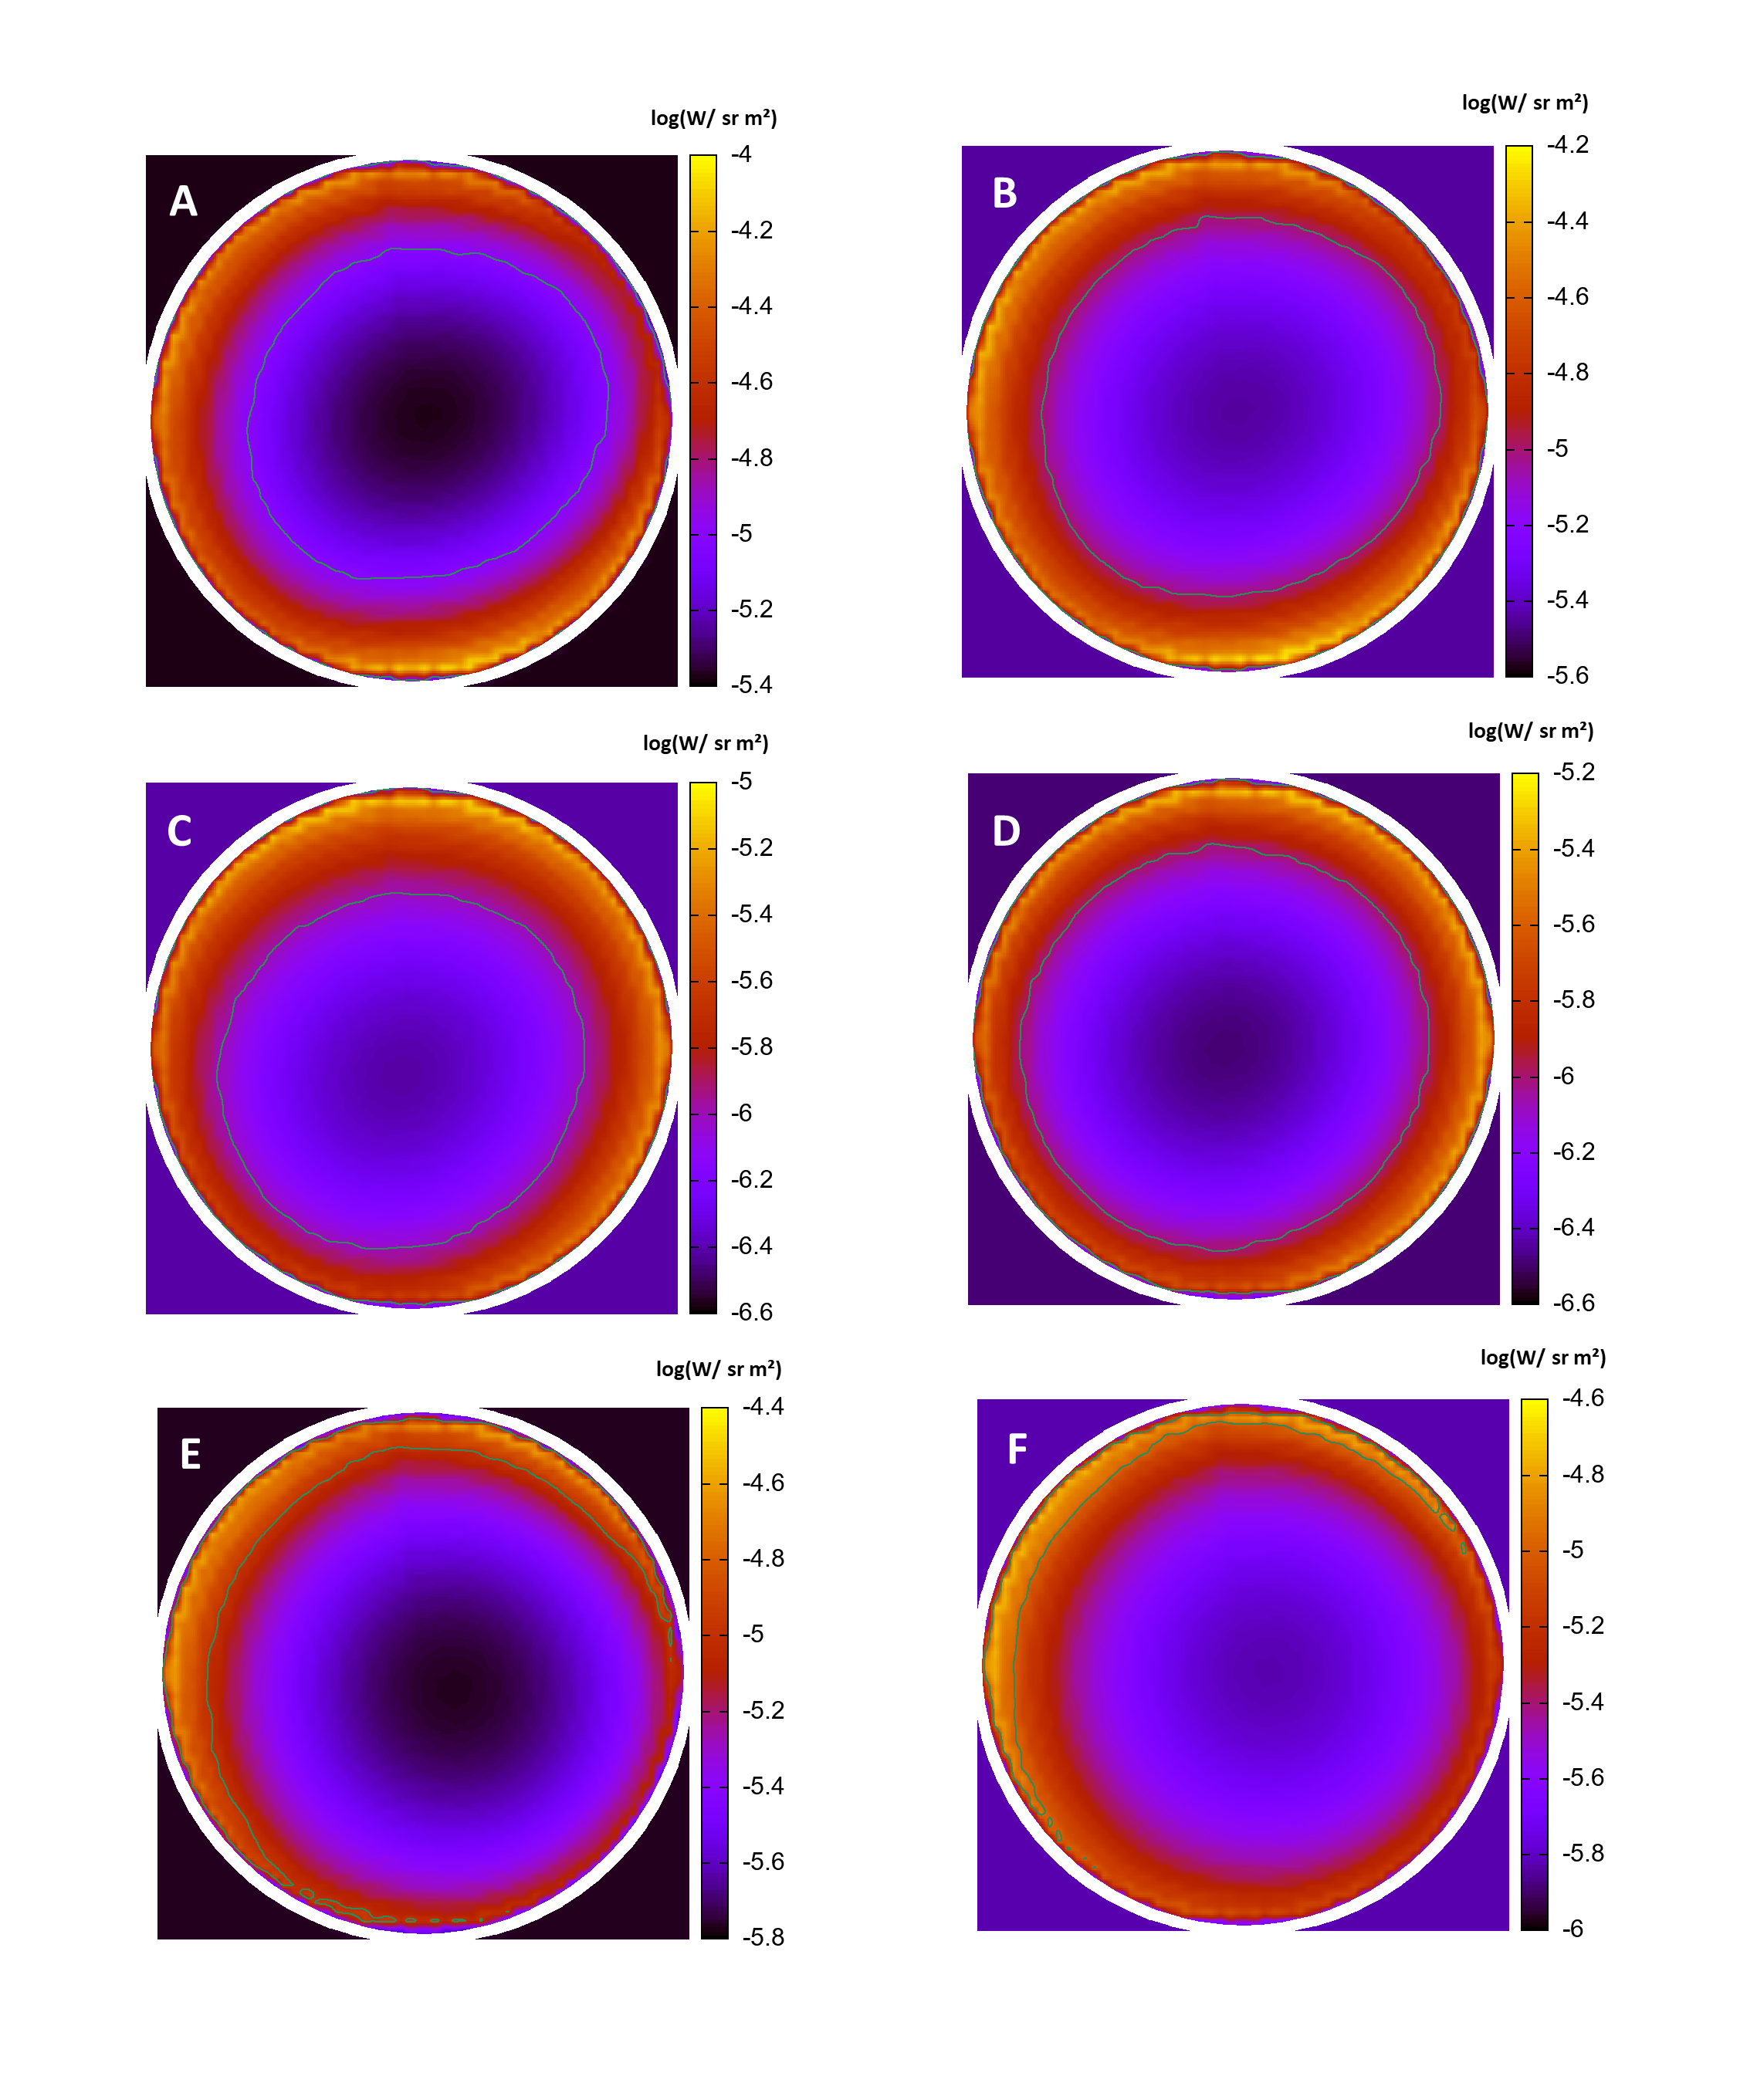
\includegraphics[width=1\textwidth]{1}
  \caption{Gráficas tipo \textit{all sky} para condiciones de cielo despejado con A) FP para GAM, B) EC para GAM, C) Caso de A) para MA, D) Caso de B) para MA, E) Caso de A) para CU y F) Caso de B) para CU} 
  \label{1}
\end{figure}


\newpage

\section{Experimentos numéricos}

Con el fin de inferir la influencia del aerosol atmosférico y la nubosidad en el brillo del cielo nocturno, se construyeron diferentes escenarios tomando como referencia la mima posición de los observadores en superficie de la sección anterior.\\

Con respecto a la influencia del aerosol atmosférico se tomaron las condiciones observadas en la climatología para la Ciudad de México (véase la \textbf{\autoref{subsubsec:propiedadesopticasaerosol}}). Para todos los casos se observa una reducción preferencial en la radiancia del horizonte en determinados ángulos acimutales con respecto a condiciones de FP. Sin embargo, en otros ángulos acimutales se tiene un aumento drástico en la radiancia en el horizonte (valores entre 2.09 x 10$^{-3}$ W sr$^{-1}$ m$^{-2}$ (en MA) y 2.72 x 10$^{-2}$ W sr$^{-1}$ m$^{-2}$ (en GAM y CU)).\\

En particular, para GAM se observa una reducción gradual en la radiancia en el cenit conforme pasan las estaciones de Invierno Seco, Primavera Seca y Temporada Lluviosa (Figura~\ref{2}), para MA se observa la misma reducción pero comenzando desde Temporada Lluviosa (Figura~\ref{3}) y, para CU comenzando desde Primavera Seca (Figura~\ref{4}). Esta diferencia en comportamiento se puede explicar remitiéndose a las funciones $\Gamma$ y $T$ del modelo que caracterizan la distribución angular de la radiancia y su atenuación atmosférica con base a la posición del observador, el AOD y $\alpha$ (parámetros que cambian significativamente en cada escenario).\\

Con respecto a la influencia de la nubosidad se observa en todos los casos una reconfiguración total de la distribución angular de la radiancia. Conforme la nube es más baja con respecto al observador los valores de randiancia aumentan drásticamente con respecto a las condiciones de FP.\\

En particular para GAM los valores extremos de radiancia aumentan de 1.83 x 10$^{-2}$ W sr$^{-1}$ m$^{-2}$ hasta 2.72 x 10$^{-2}$ W sr$^{-1}$ m$^{-2}$ (Figura~\ref{5}). Para MA de 6.73 x 10$^{-3}$ W sr$^{-1}$ m$^{-2}$ a 1.49 x 10$^{-2}$ W sr$^{-1}$ m$^{-2}$ (Figura~\ref{6}) y para CU de 1.22 x 10$^{-2}$ W sr$^{-1}$ m$^{-2}$ a 2.47 x 10$^{-2}$ W sr$^{-1}$ m$^{-2}$ (Figura~\ref{7}). Resultan interesantes los casos de MA y CU en que la nubosidad crea un efecto de enmascaramiento de radiancia en regiones del horizonte de donde proviene menos luz.\\

Como se aborda en la  \textbf{\autoref{subsec:tendenciasradiancia}} por el potencial ahorro económico que supone, mundialmente se está llevando a cabo una sustitución de instalaciones de alumbrado público cambiando fuentes tradicionales a LED. Entre otros motivos que tienen que ver con la susceptibilidad de un gran número de organismos a las longitudes de onda corta, los LEDs son la fuente de luz con mayor potencial en términos de CL ya que las longitudes de onda corta que emite se transportan más eficientemente en la atmósfera por acción de la dispersión de Rayleigh.\\

En la Figura~\ref{8} se observa que al simular el cambio de iluminación de la ciudad a LED, en todos los casos ocurre un marcado aumento en los valores de radiancia con respecto a las condiciones de FP.\\

\newpage

\subsection{Influencia del aerosol atmosférico en la distribución de radiancia}

\begin{figure}[H]
  \centering
    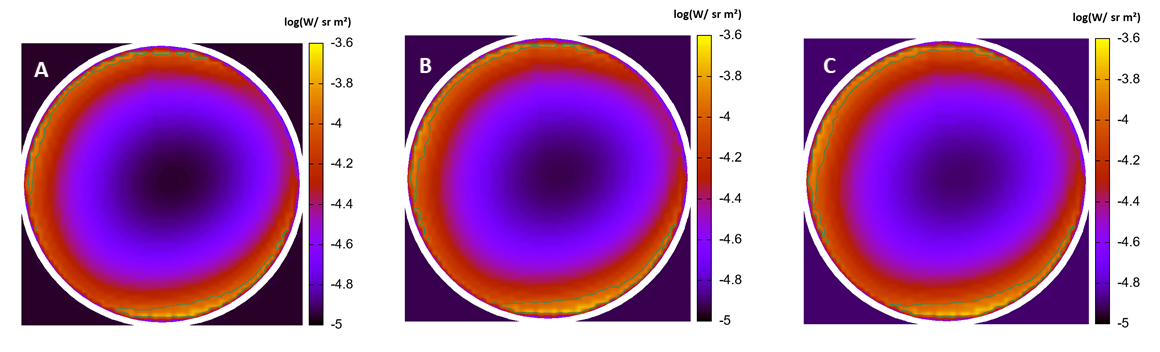
\includegraphics[width=1\textwidth]{2}
  \caption{Gráficas tipo \textit{all sky} para condiciones de cielo despejado para GAM en A) Invierno Seco, B) Primavera Seca y C) Temporada Lluviosa} 
  \label{2}
\end{figure}}

\begin{figure}[H]
  \centering
    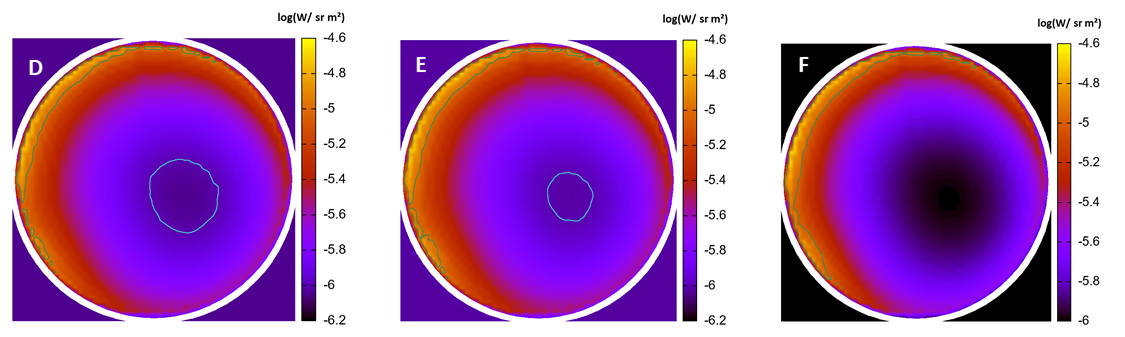
\includegraphics[width=1\textwidth]{3}
  \caption{Gráficas tipo \textit{all sky} para condiciones de cielo despejado para MA en A) Invierno Seco, B) Primavera Seca y C) Temporada Lluviosa} 
  \label{3}
\end{figure}

\begin{figure}[H]
  \centering
    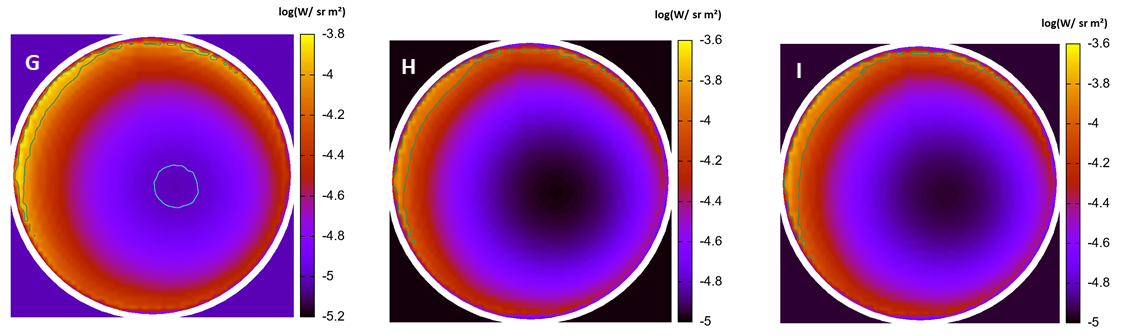
\includegraphics[width=1\textwidth]{4}
  \caption{Gráficas tipo \textit{all sky} para condiciones de cielo despejado para CU en A) Invierno Seco, B) Primavera Seca y C) Temporada Lluviosa} 
  \label{4}
\end{figure}

\newpage

\subsection{Influencia de la nubosidad en la distribución de radiancia}

\begin{figure}[H]
  \centering
    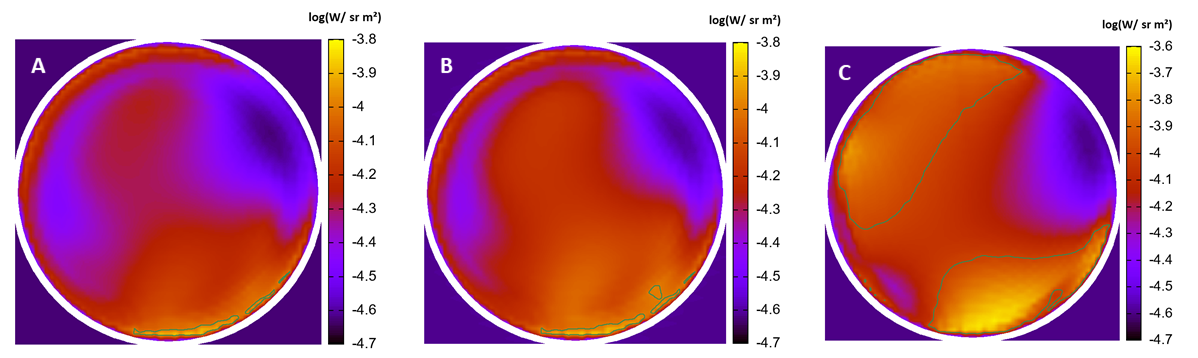
\includegraphics[width=1\textwidth]{5}
  \caption{Gráficas tipo \textit{all sky} para condiciones de cielo nublado para GAM con A) \textit{altocumulus}, B) \textit{altostratus} y C) \textit{stratus}} 
  \label{5}
\end{figure}

\begin{figure}[H]
  \centering
    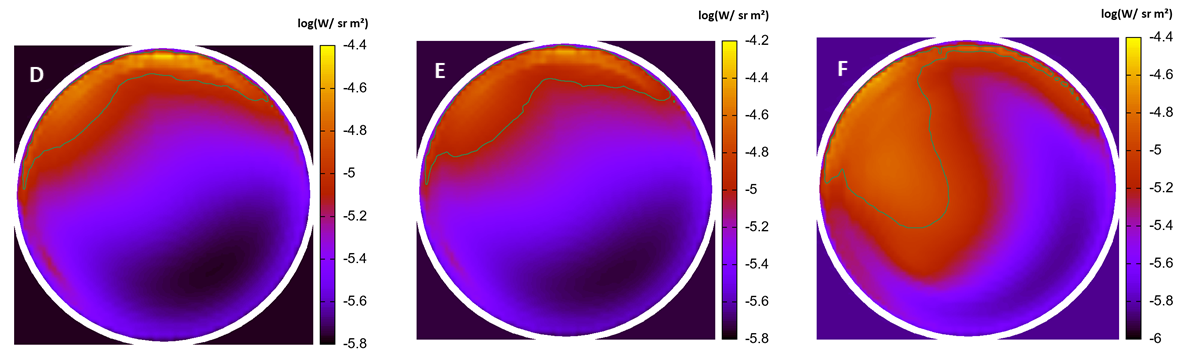
\includegraphics[width=1\textwidth]{6}
  \caption{Gráficas tipo \textit{all sky} para condiciones de cielo nublado para MA con A) \textit{altocumulus}, B)  \textit{altostratus} y C) \textit{stratus}} 
  \label{6}
\end{figure}

\begin{figure}[H]
  \centering
    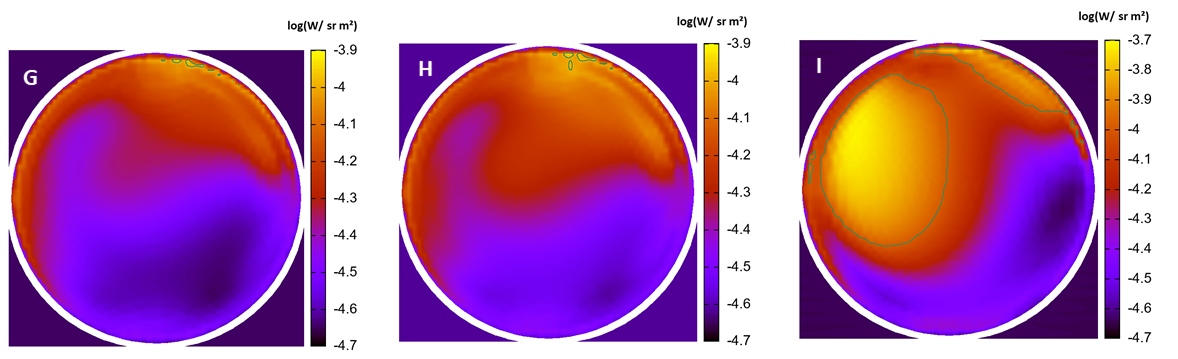
\includegraphics[width=1\textwidth]{7}
  \caption{Gráficas tipo \textit{all sky} para condiciones de cielo nublado para CU con A) \textit{altocumulus}, B) \textit{altostratus} y C) \textit{stratus}} 
  \label{7}
\end{figure}

\newpage

\subsection{Cambio del tipo de luminarias en la Ciudad de México}

\begin{figure}[H]
  \centering
    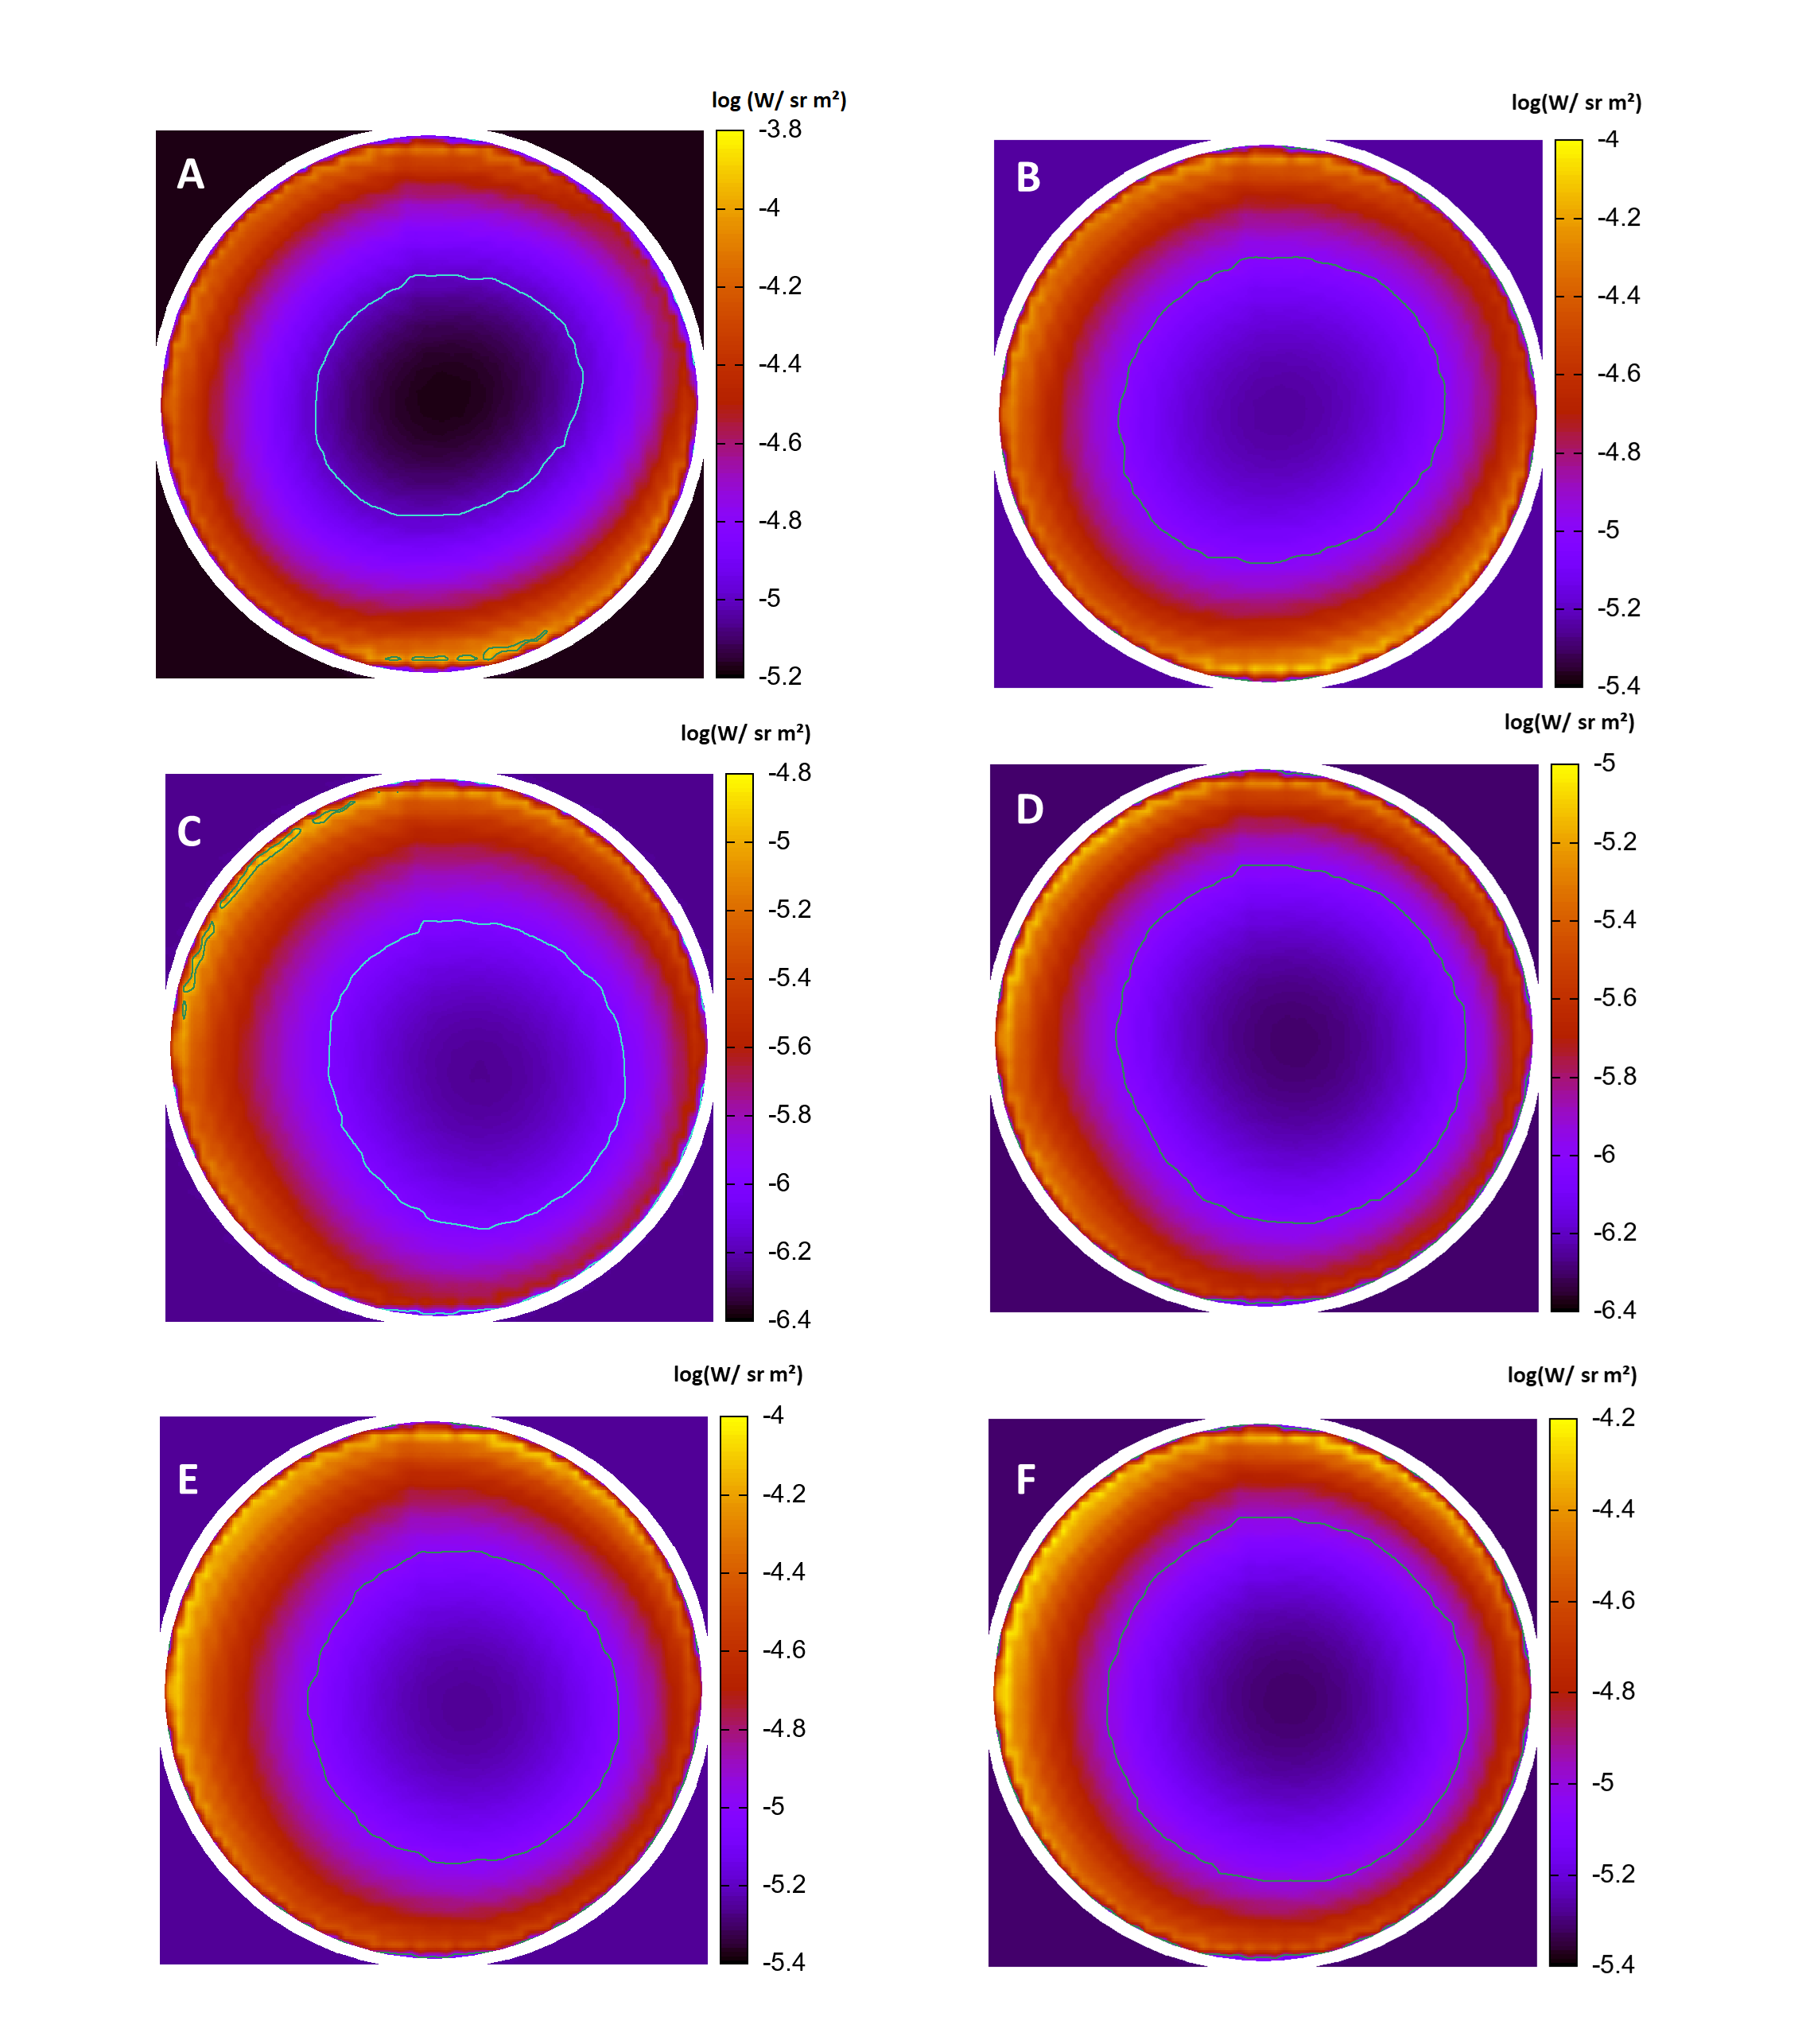
\includegraphics[width=1\textwidth]{8}
  \caption{Gráficas tipo \textit{all sky} para condiciones de cielo despejado con tipo de luminaria LED con A) FP para GAM, B) EC para GAM, C) Caso de A) para MA, D) Caso de B) para MA, E) Caso de A) para CU y F) Caso de B) para CU} 
  \label{8}
\end{figure}

\newpage

\section{Mapa CL-CDMX}
\label{sec:mapacl}

Para efectos de evaluación teórica de los efectos de la distribución de radiancia en el cielo nocturno (brillo del cielo) sobre la irradiancia difusa percibida por un observador en superficie se construyó el \textbf{Mapa Teórico de Contaminación Lumínica de la Ciudad de México} con las salidas del modelo \textit{SkyGlow} (Figura~\ref{8}).\\

Advertencia: los valores de irradiancia presentados en el mapa no son un indicativo directo de los niveles de CL, más bien, son representativos de la tendencia de CL en el rango visible del EE. De manera tradicional los efectos directos de la CL sobre la biodiversidad se efectúan empleando mediciones fotométricas que quedan restringidas en el ámbito de la visión humana y, por lo tanto, se pierde mucha información en el proceso; un aspecto novedoso que ofrece la base teórica del Mapa CL-CDMX es la posibilidad de mapear valores de irradiancia en superficie aplicando filtros específicos basados en la visión de diferentes especies, es decir: generar mapas de cómo perciben el brillo del cielo nocturno diferentes especies en diferentes lugares de la ciudad.\\

Lo anterior es posible efectuarlo de acuerdo con \cite{Solano2013} a través de la modificación de la ecuación \ref{eq:2.5} obteniendo:

\begin{equation}
D_{\lambda} = \int_{\lambda_{1}}^{\lambda_{1}} \zeta(\lambda) \int_{z = 0}^{z =\pi/2} \int_{\phi = 0}^{\phi = 2\pi} I_{\lambda} (z, \phi) \: sen \,z \: dz \: d\phi
\end{equation}\\


En donde $\zeta(\lambda)$ es la respuesta espectral de una especie en particular siendo una función de su tipo de visión (fotópica, mesópica o escotópica).\\

Por otro lado, el Mapa CL-CDMX permite evaluar la correcta reproducción de las tendencias observadas de CL por la DNB (Figura~\ref{radiancetrends}). En general, se observa una reproducción muy fiel al tener los niveles más bajos de irradiancia fuera de la ciudad y los mayores en el Centro de la ciudad integrado por los Sectores Centro, Roma, Tlatelolco, Buenavista y Morelos. Nótese que las regiones en color blanco corresponden a zonas no iluminadas, como el sur de la Ciudad de México y ANPs dentro de la ciudad, o con iluminación especial (no correspondiente al alumbrado público) como el Aeropuerto Internacional de la Ciudad de México, CU, Reclusorio Norte y el Colegio Militar.\\

El Mapa CL-CDMX se inscribe como un antecedente para la zonificación que necesita cualquier legislación en materia de CL (véase la \textbf{\autoref{subsec:marcoregulatorio}}). Tal zonificación tiene que estar basada en el enfoque socioecosistémico abordado en la \textbf{\autoref{subsec:enfoquesocioecosistemico}}: no porque una zona sea altamente comercial o turística significa que sus fuentes de luz puedan ser de cualquier tipo o derrochar energía, tiene que pensarse en que la especie humana coexiste con otras miles de especies en un mismo espacio y que nuestros caminos y calles son los suyos también; la sustentabilidad no sólo se construye para el futuro sino para hoy también, las ciudades no son estructuras inmutables que tengan que reproducir esquemas antropocentristas sino procesos de la naturaleza. 

\newpage

\vspace{100mm} 

\begin{figure}[H]
  \centering
    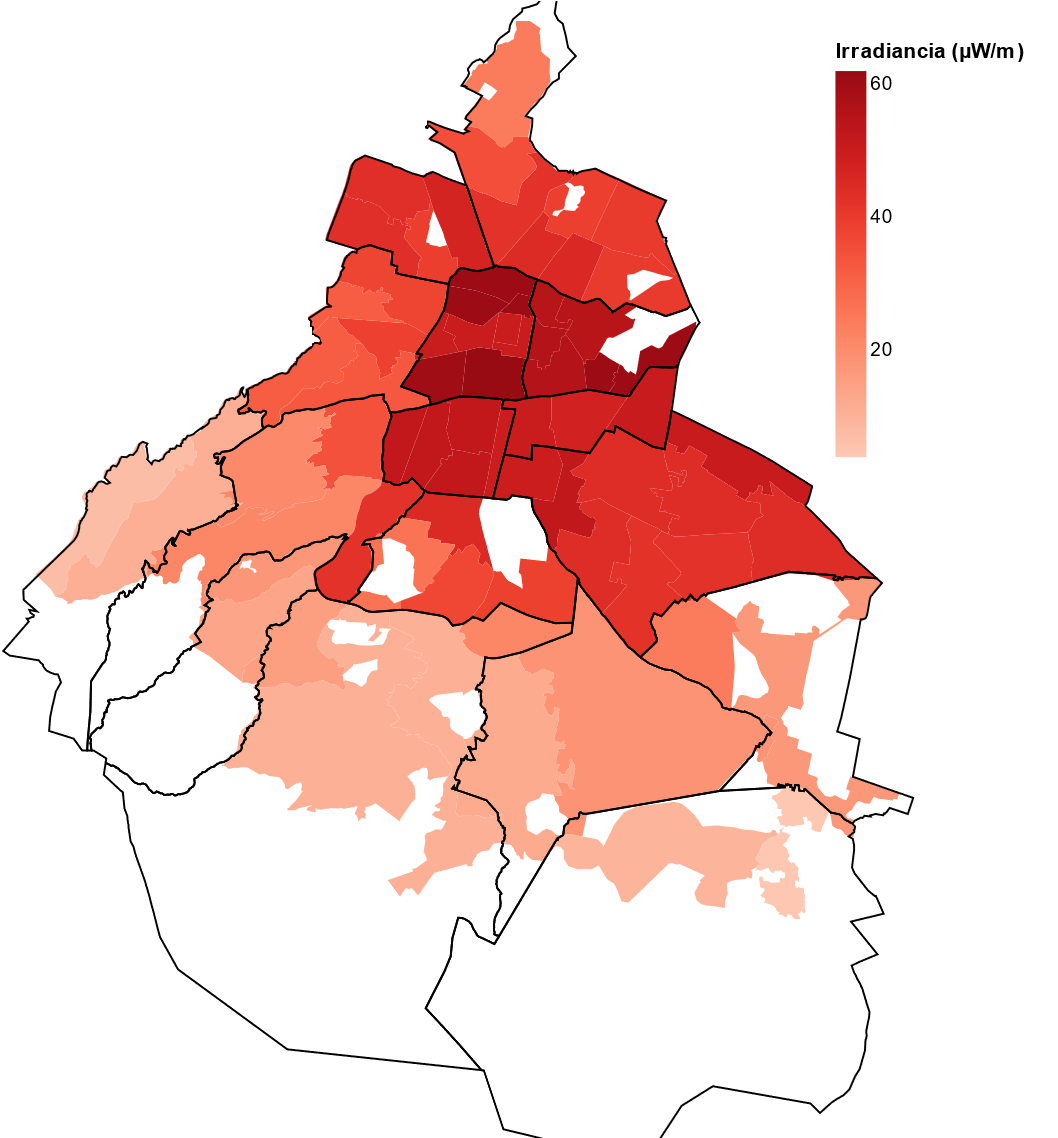
\includegraphics[width=1\textwidth]{MapaCLCDMX}
  \caption{Mapa CL-CDMX} 
  \label{MapaCLDMX}
\end{figure}

\newpage
	
	\chapter{Conclusiones}
\label{chap:conclusiones}

\begin{enumerate}[I]

\item Se logró reproducir con éxito el modelo \textit{SkyGlow} para el caso de la Ciudad de México lo cual permitió generar los productos \textbf{Mapa CL-CDMX} que se inscribe como el primer antecedente a tomar en cuenta para la mitigación de la CL a través de la zonificación de la iluminación pública en la Ciudad de México, y las \textbf{gráficas tipo all sky} que permitieron comprobar que el aerosol atmosférico y la nubosidad son los principales moduladores del brillo del cielo nocturno. El modelo se configuró para reproducir prácticamente cualquier escenario atmosférico para un observador situado en cualquier punto de la ciudad.

\item Se construyó el \textbf{Inventario de Alumbrado Público de la Ciudad de México} con datos públicos que de otra manera no habrían podido estudiarse en conjunto por la marcada separación que existe entre las oficinas de transparencia de las diferentes alcaldías de la ciudad. Con estos datos no sólo se alimentó el modelo sino además se efectuaron cálculos que indican que el consumo de energía eléctrica en la Ciudad de México es responsable del 6\% de las emisiones nacionales anuales de CO$_2$.

\item Se comprobó que uno de los factores más críticos a considerar para estimar el potencial efecto en la CL de las fuentes de luz es su dependencia espectral. Se comprobó teóricamente que el cambio de sistema de iluminación actual de la ciudad (halogenuros metálicos) a LED podría aumentar marcadamente los patrones del brillo del cielo nocturno. 

\item En mayor o menor medida se encontró presencia de CL en todo el territorio de la Ciudad de México. Alcaldías como Gustavo A. Madero, Venustiano Carranza, Benito Juárez, Cuauhtémoc, Iztacalco son las más contaminadas con valores de radiancia de hasta 86 nW sr$^{-1}$ cm$^{-2}$ mientras que Milpa Alta, Cuajimalpa de Morelos, Tlalpan, Tláhuac y Magdalena Contreras registran valores mínimos de hasta 6 nW sr$^{-1}$ cm$^{-2}$. Espacios naturales embebidos en la ciudad como la REPSA de la Universidad Nacional Autónoma de México también son afectados por CL.

\end{enumerate}
	
	\chapter{Recomendaciones}

Los resultados de este trabajo van encaminados a la legislación y técnicas de iluminación conociendo qué tipo de fuentes resultan más contaminantes. 
	
	\phantomsection
	\renewcommand\bibname{Referencias}
	\addcontentsline{toc}{chapter}{Referencias}
	\bibliography{referencias}
	
\end{document}